%%%%%%%%%%%%%%%%%%%%%%%%%%%%%%%%%%%%%%%%%

\chapter{The LANL nEDM experiment}\label{chap:LANL_nEDM}

%%%%%%%%%%%%%%%%%%%%%%%%%%%%%%%%%%%%%%%%%

At the Los Alamos National Laboratory (LANL), a solid deuterium (SD$_2$) based superthermal UCN source coupled to a spallation target has been providing UCN to experiments for the last 20 years (Fig.~\ref{fig:AreaB_schematic}). The UCN source (Sec.~\ref{sec:lanl_ucn_source}) was upgraded to host a new nEDM experiment that will use Ramsey's method of separated oscillatory fields to search for the nEDM with an uncertainty goal of $\delta \gls*{d_n} = 2.7\times 10^{-27}$~$e\cdot\text{cm}$ (Sec.~\ref{sec:lanl_nedm_uncertainty}).

The envisioned LANL nEDM experiment (Fig.~\ref{fig:envisioned_lanl_nedm}) will include features such as:
%
\begin{itemize}
    \item Two precession cells (Sec.~\ref{sec:precession_cells})
    \item Simultaneous spin analyzers (Sec.~\ref{sec:spin_flipper_analyzer})
    \item An external array of optically pumped magnetometers (Sec.~\ref{sec:magnetic_field_req})
    \item A \hg comagnetometer (Sec.~\ref{sec:199hg_comag}) and external \hg magnetometers
\end{itemize}

In this chapter we provide an overview of LANL nEDM instrumentation, and review some of the main systematic effects limiting the sensitivity of nEDM measurements.

%%%%%%%%%%%%%%%%%%%%%%%%%%%%%%%%%%%%%%%%%

\section{Principles of an nEDM measurement}\label{sec:principles_nEDM}

%%%%%%%%%%%%%%%%%%%%%%%%%%%%%%%%%%%%%%%%%

A measurement cycle in the envisioned LANL nEDM experiment consists of the following steps: 
%
\begin{enumerate}
    \item Polarized \ucn are loaded into precession cell(s), in a region where a static magnetic $\vv{B}_0$ and electric field $\vv{E}$ are applied. $\vv{B}_0$ and $\vv{E}$ are in either a parallel ($\uparrow\uparrow$) or antiparallel ($\uparrow\downarrow$) configuration.
    \item The Ramsey sequence (Sec.~\ref{sec:ramsey-method}) is applied to generate a point on a Ramsey fringe, which is necessary for determination of UCN precession frequency in both parallel and antiparallel configurations.
    \item \ucn are unloaded from the precession cell(s) to be detected and to have their final spin state analyzed.
\end{enumerate}
%
Measurement cycles are repeated many times to minimize statistical uncertainty (Sec.~\ref{sec:figure_of_merit}). The Ramsey fringe is then fit to determine neutron precession frequency in a configuration. In the absence of any systematic effects, any difference in neutron precession frequency $\omega_\text{n}$ between the $\vv{B}_0\uparrow\uparrow\vv{E}$ and $\vv{B}_0\uparrow\downarrow\vv{E}$ modes indicates the existence of a nonzero electric dipole moment \gls*{d_n}. This is written as
%
\begin{gather}
    \omega_\text{n}^{\uparrow\uparrow} - \omega_\text{n}^{\uparrow\downarrow} = -\frac{4\gls*{d_n}E}{\hbar}\label{eq:delta_omega_dipole_relation}
\end{gather}
%
where
%
\begin{align}
    \hbar \omega_\text{n}^{\uparrow\uparrow} &= -2\gls{mu_n}B_0 - 2\gls*{d_n}E\\
    \hbar \omega_\text{n}^{\uparrow\downarrow} &= -2\gls{mu_n}B_0 + 2\gls*{d_n}E
\end{align}
%
In the case where $B_0$ and $E$ differ between configurations,
%
\begin{gather}
    \gls*{d_n}=\frac{\hbar(\omega_\text{n}^{\uparrow\uparrow} - \omega_\text{n}^{\uparrow\downarrow})-2\gls{mu_n}(B_0^{\uparrow\uparrow} - B_0^{\uparrow\downarrow})}{2\hbar(E^{\uparrow\uparrow} - E^{\uparrow\downarrow})}
\end{gather}
%
\begin{figure}
    \centering
    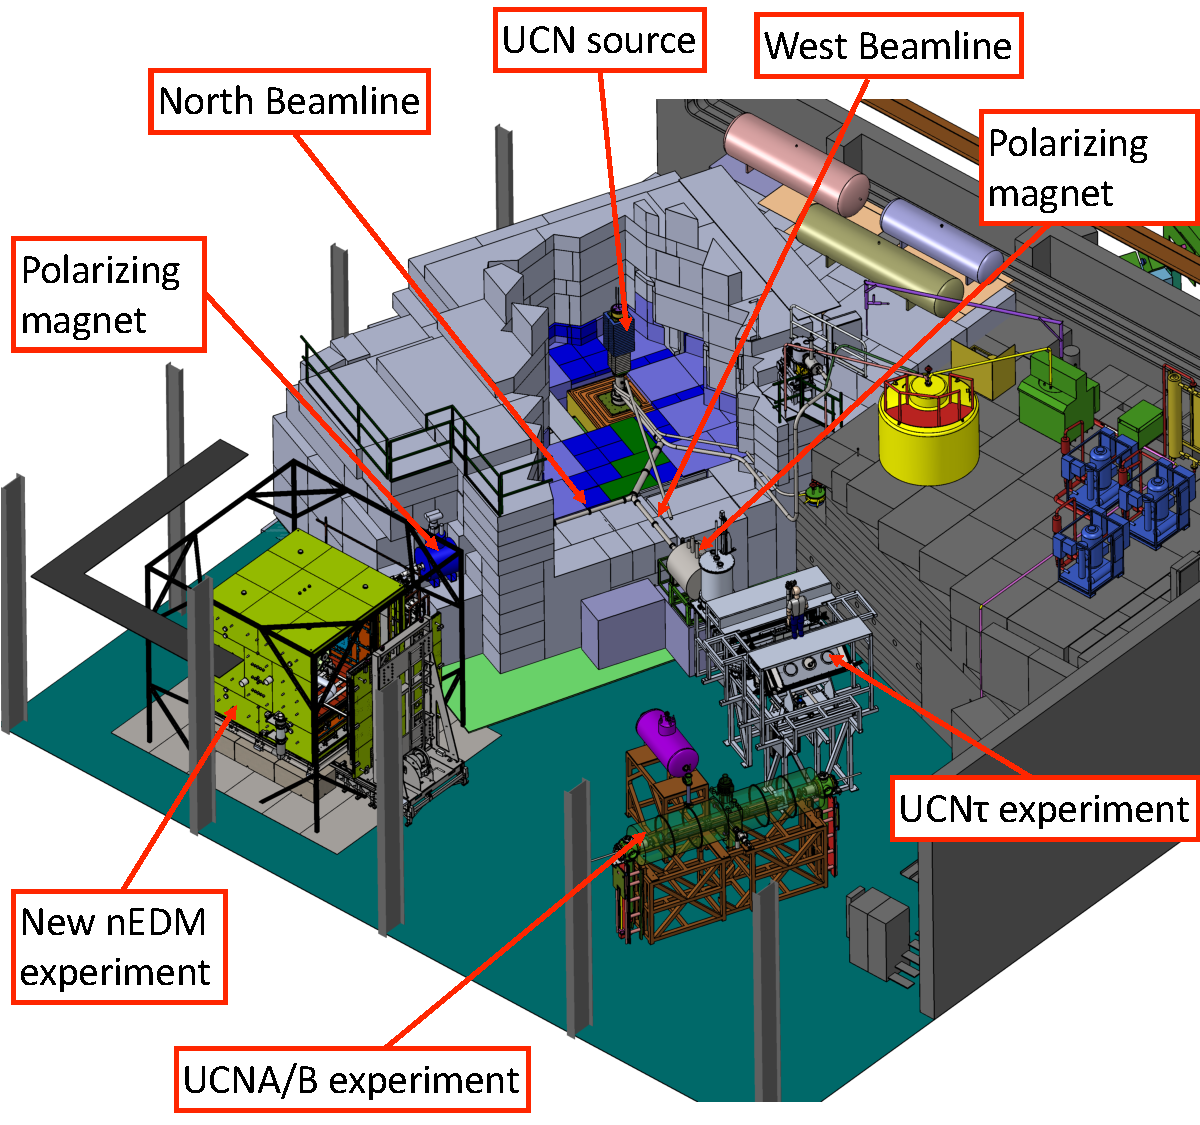
\includegraphics[width=0.6 \textwidth]{AreaB_v3.pdf}
    \caption{Schematic of the experimental area at the LANL UCN facility}
    \label{fig:AreaB_schematic}
\end{figure}

\begin{figure}
    \centering
    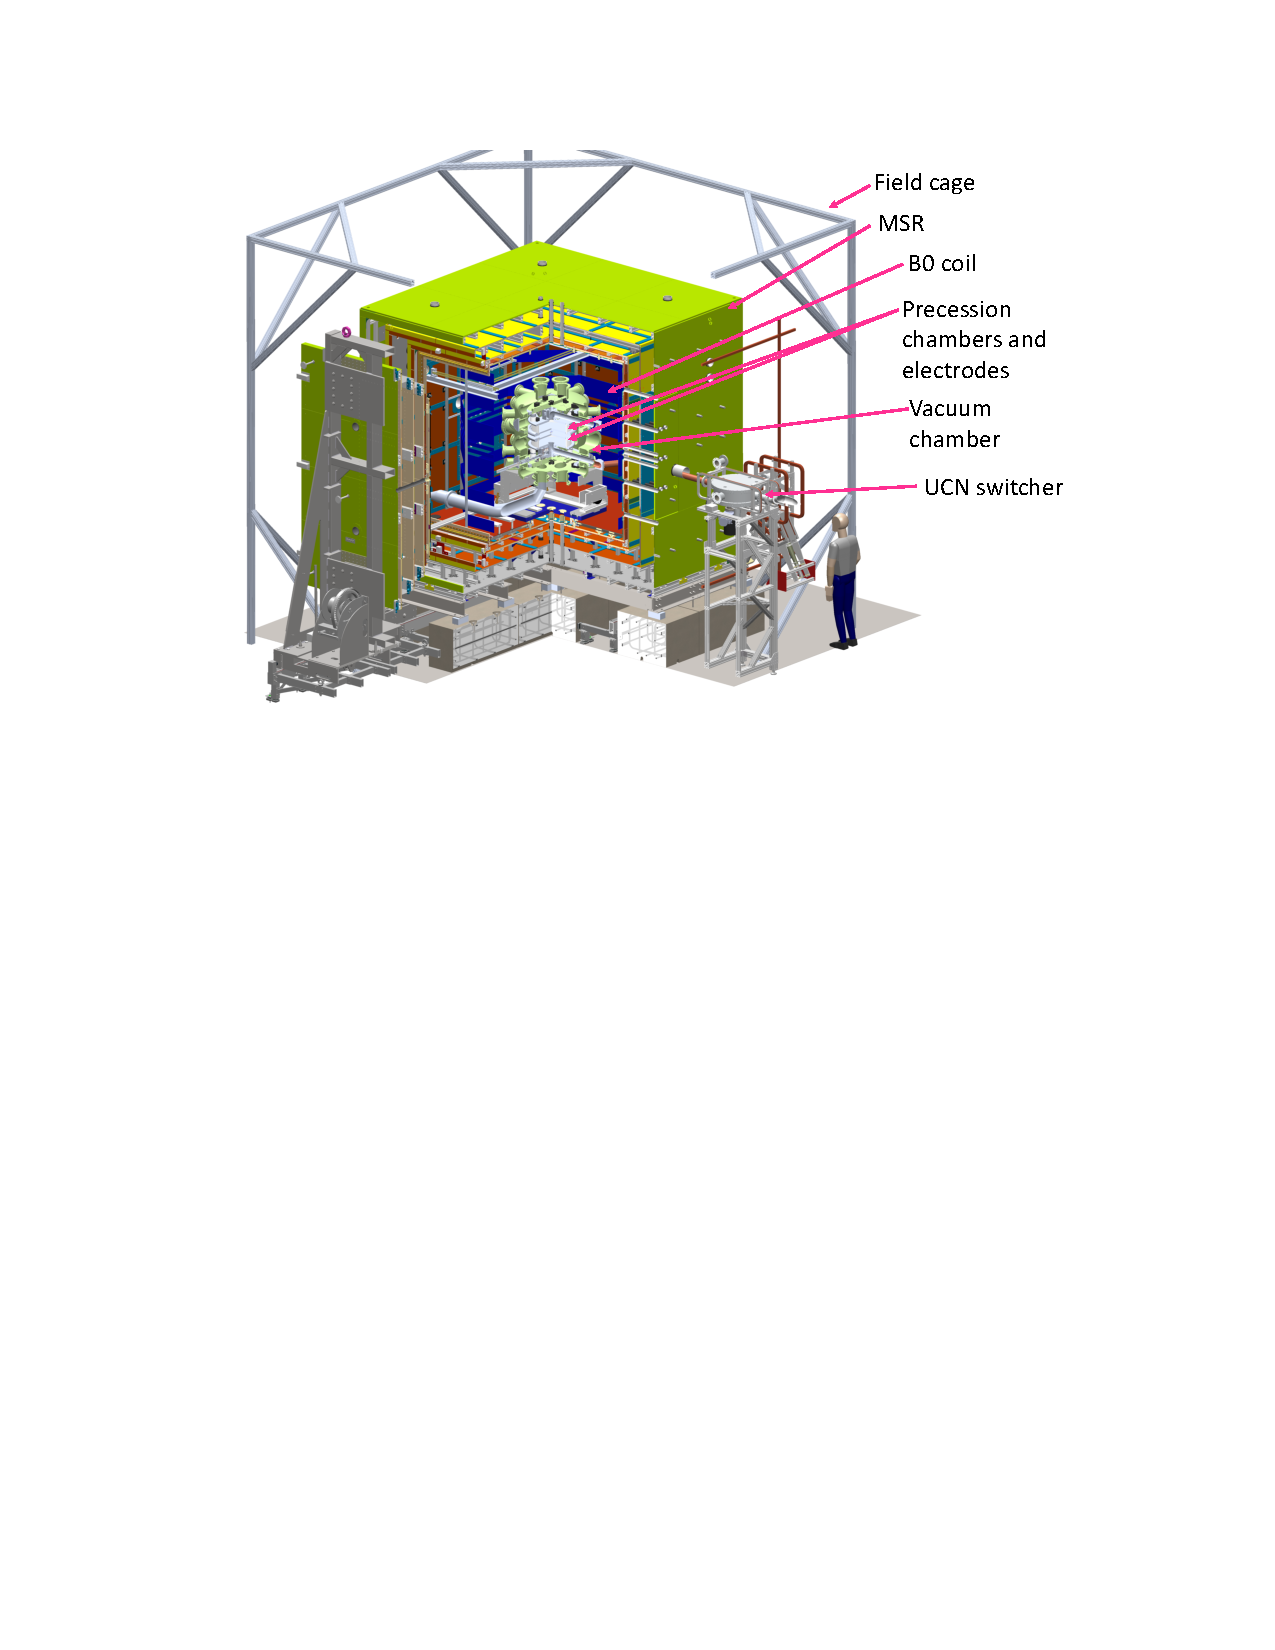
\includegraphics[width=0.9\textwidth]{figures/envisioned_lanl_nedm.pdf}
    \caption{Model of the LANL nEDM experiment}
    \label{fig:envisioned_lanl_nedm}
\end{figure}

%%%%%%%%%%%%%%%%%%%%%%%%%%%%%%%%%%%%%%%%%

\section{Statistical uncertainty figure of merit}\label{sec:figure_of_merit}

%%%%%%%%%%%%%%%%%%%%%%%%%%%%%%%%%%%%%%%%%

Equation~7.28 from Ref.~\cite{golubUCN} gives the number of neutrons counted in a single Ramsey sequence as
%
\begin{gather}
    N_\text{R}(\Delta \omega) = N \left( 1 - \gls*{alpha} \cos \,\Delta \omega \, \gls*{T_fp} \right)/2
\end{gather}
%
where \gls*{alpha} is the spin contrast of a Ramsey fringe, defined by Eq.~(\ref{eq:alpha}), and $\gls*{T_fp}$ is the free precession period of the Ramsey method. A nonzero nEDM causes an interaction with $\vv{E}$ that produces a precession frequency shift $\Delta\omega=\omega-\omega_0$, where $\omega$ is the applied RF frequency and $\omega_0$ is defined by Eq.~(\ref{eq:larmor_freq}). 

To maximize sensitivity to small shifts in the resonant frequency, we examine where the slope of the central fringe is largest
%
\begin{gather}
    \frac{\partial N_\text{R}(\Delta \omega)}{\partial \, \Delta \omega} = N \frac{\alpha}{2} \gls*{T_fp} \sin \, \Delta \omega \, \gls*{T_fp} \label{eq:slope_ramsey}
\end{gather}
%
The error of $\Delta \omega$ is given by
%
\begin{gather}
    \sigma(\Delta \omega) = \frac{\partial \, \Delta \omega}{\partial N_\text{R}(\Delta \omega)}\delta N_\text{R}(\Delta \omega) = \frac{\partial \, \Delta \omega}{\partial N_\text{R}(\Delta \omega)} \sqrt{N}
    \label{eq:sigma_delta_omega}
\end{gather}
%
Using Eq.~(\ref{eq:slope_ramsey}) where $\Delta \omega \, \gls*{T_fp} = \pi/2$ (for the largest slope), Eq.~(\ref{eq:sigma_delta_omega}) becomes
%
\begin{gather}
    \sigma(\Delta \omega) = \frac{2}{\gls*{alpha} \gls*{T_fp} \sqrt{N}}
\end{gather}
%
From reversal of the electric field, Eq.~(\ref{eq:delta_omega_dipole_relation}), we remove the dependence on $\Delta\omega$ to obtain
%
\begin{gather}
    \sigma_{\gls*{d_n}} = \frac{\hbar}{2\gls*{alpha} E \gls*{T_fp} \sqrt{N}}\label{eq:figure_of_merit}
\end{gather}
%
This is the figure of merit for an nEDM experiment using the Ramsey method. \gls{hbar} is Planck’s constant, \gls{alpha} is a factor describing the spin contrast of a Ramsey fringe, $N$ is the number of the detected UCN, and $E$ is the strength of the applied electric field.

%%%%%%%%%%%%%%%%%%%%%%%%%%%%%%%%%%%%%%%%%

\subsection
{
    \texorpdfstring{Statistical Uncertainty of the \acrshort{lanl} \acrshort{nedm}}
                    {Statistical Uncertainty of the LANL nEDM}\label{sec:lanl_nedm_uncertainty}
}

%%%%%%%%%%%%%%%%%%%%%%%%%%%%%%%%%%%%%%%%%

The nominal run parameters for the LANL nEDM relevant to the estimate of uncertainty are $\gls*{T_fp}=180\text{ s and } E=12\text{ kV/cm}$. As will be shown in Chap.~\ref{chap:north_beamline_paper}, we have measured $N=60\,000\text{ UCN}$ in a protype cell. We let $\gls*{alpha}=0.8$, as was achieved in Ref.~\cite{ABE20}.

Using Eq.~(\ref{eq:figure_of_merit}), the uncertainty per cell per run is $7.8 \times 10^{-25}e\cdot\text{cm}$. For a full day of measurements (assuming a \qty{300}{\s} duty cycle with two precession cells), we have $N_\text{day}=2\times60\,000\times86\,400\text{ (seconds in a day)}/300$ and $\sigma_{\gls*{d_n}}=3.24\times10^{-26}e\cdot\text{cm}$. A year of continuous running gives $N_\text{year}=365\times N_\text{day}$ and $\sigma_{\gls*{d_n}}=1.7\times10^{-27}e\cdot\text{cm}$. At a 90\% confidence level, the uncertainty is multiplied by an additional factor of $1.6$, giving
%
\begin{gather}
    \sigma_{\gls*{d_n}}=2.71\times10^{-27}e\cdot\text{cm (90\% \acrshort{cl})}
\end{gather}
%
With an assumed data taking efficiency of 50\% (for experiment down time, calibration and systematic studies) and the accelerator production schedule at LANL, this uncertainty would be reached in 5 calendar years.

%%%%%%%%%%%%%%%%%%%%%%%%%%%%%%%%%%%%%%%%%

\section
{
    \texorpdfstring{UCN production at \acrshort{lanl}}
                   {UCN production at LANL}
}\label{sec:lanl_ucn_source}

%%%%%%%%%%%%%%%%%%%%%%%%%%%%%%%%%%%%%%%%%

\begin{figure}
    \centering
    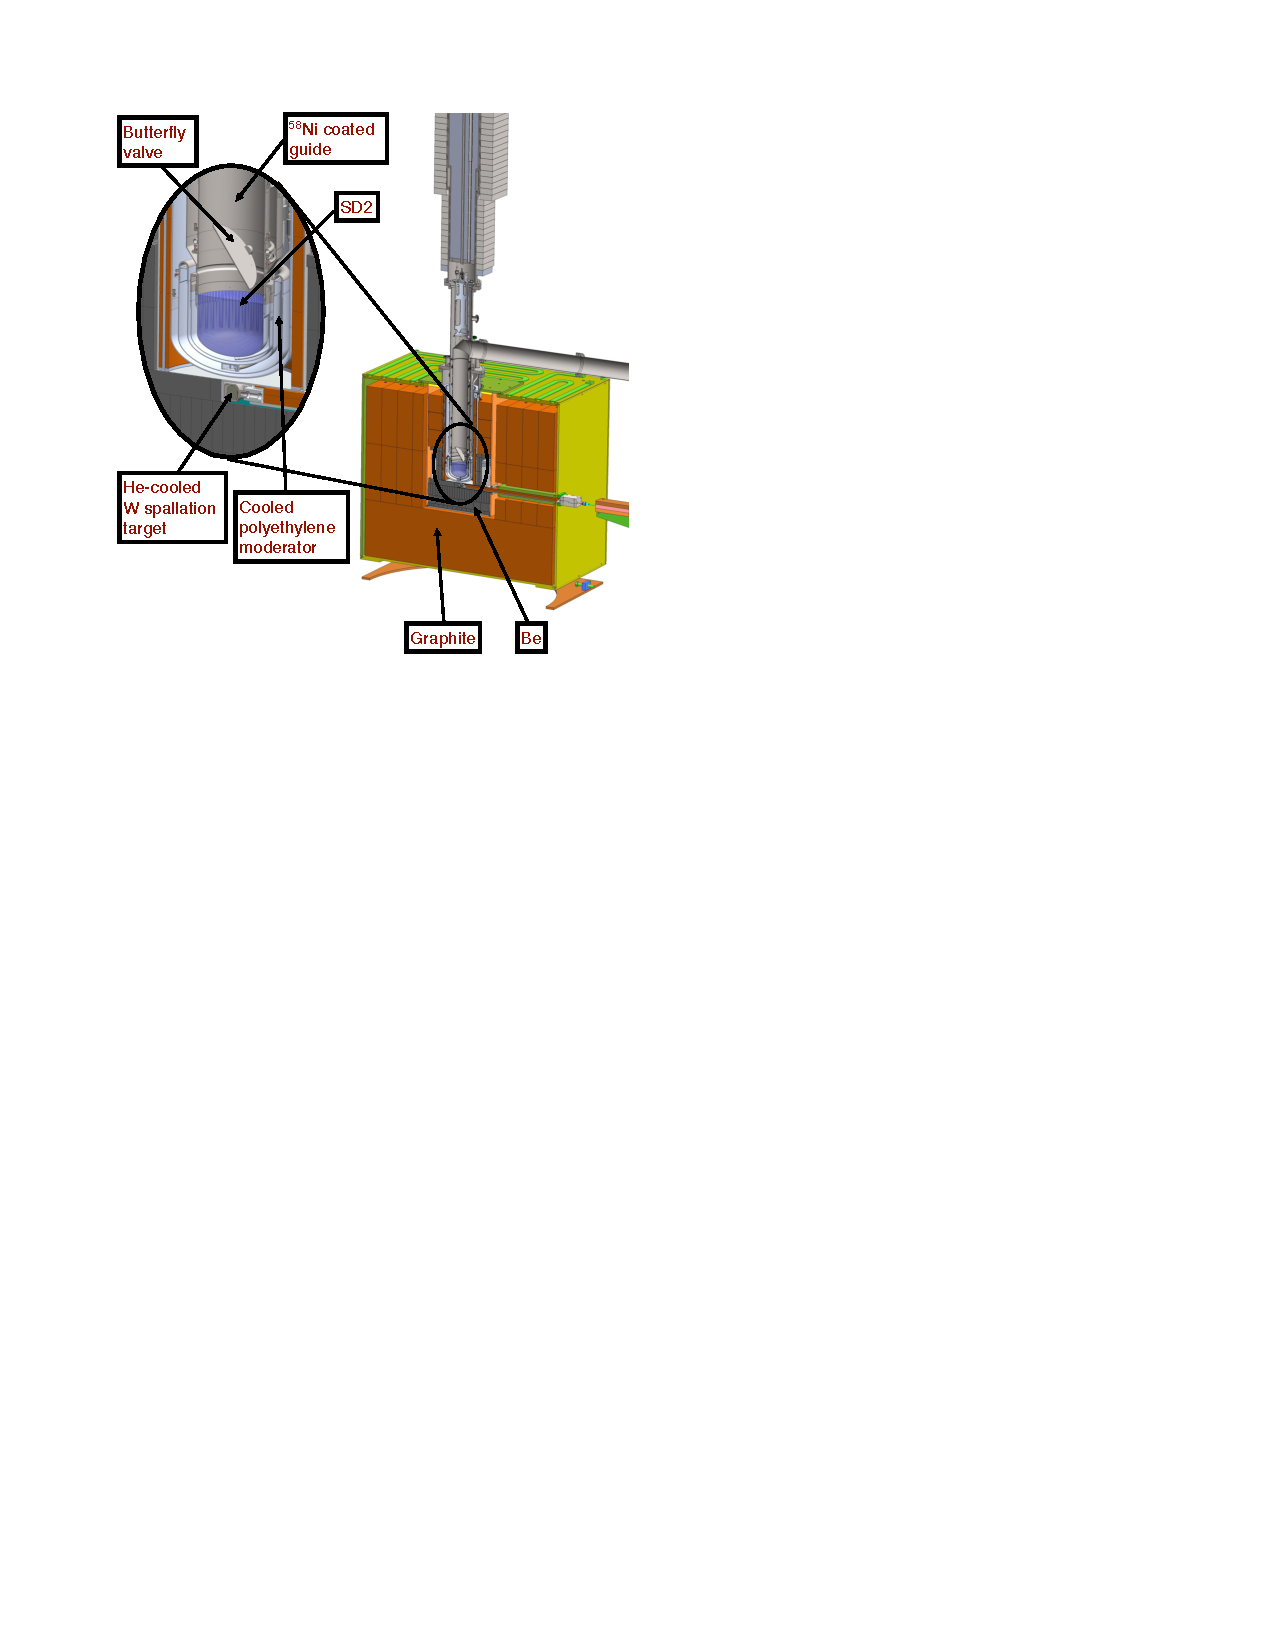
\includegraphics[width=0.6 \textwidth]{figures/lanl_ucn_source.pdf}
    \caption[Cutaway view of the LANL UCN source]
    {Cutaway view of the LANL UCN source. Image adapted from Ref.~\cite{ito_performance_2018}}
    \label{fig:lanl_ucn_source}
\end{figure}

At LANL, neutrons are produced by a pulsed \qty{800}{M\eV} proton beam incident on a tungsten target, which is surrounded by ambient temperature beryllium and graphite. The spallation neutrons are converted to cold neutrons by polyethylene bead moderators, then converted to UCN by downscattering within an SD$_2$ crystal~\cite{saunders_performance_2013}.

As in Fig.~\ref{fig:lanl_ucn_source}, UCN leaving the SD$_2$ crystal are directed upwards along a \qty{1}{\meter} vertical guide coated in $\ce{^{58}Ni}$, to account for a Snell's law \qty{100}{\nano\eV} boost (Sec.~\ref{sec:ucn_reflection_transmission}). The UCN are then transported \qty{6}{\meter} along a horizontal NiP coated stainless steel guide to the exit of the biological shield~\cite{ito_performance_2018}.

A butterfly valve near the bottom of the vertical guide reduces the probability of UCN returning to the SD$_2$ and being absorbed. The valve is open while proton beam pulses are delivered to the spallation target and closed otherwise. The proton current from the accelerator is delivered in packets of 10 pulses, of pulse width \qty{625}{\micro\s} at \qty{20}{\hertz}, with a gap between packets of \qty{5}{\s}. The average current delivered to the target is $\sim\qty{9}{\micro A}$.

In a 2017 source upgrade, the cryogenic insert, which housed the SD$_2$ converter as well as the cold neutron moderator, was replaced with an improved design. The upgrade produced a factor of four increase in UCN density. UCN density measured at the exit of the biological shield was $\qty{184(32)}{UCN\per \cm^3}$, and polarized UCN density stored in an external cell was $\qty{39(7)}{UCN\per \cm^3}$~\cite{ito_performance_2018}.

With the upgrade, a new UCN beamline (called the North Beamline) was constructed for the new nEDM experiment (Fig.~\ref{fig:AreaB_schematic}). Measurements and analysis characterizing the performance of the North Beamline are presented in Chap.~\ref{chap:north_beamline_paper}.


%%%%%%%%%%%%%%%%%%%%%%%%%%%%%%%%%%%%%%%%%

\section
{
    Magnetic field uniformity and stability requirements\label{sec:magnetic_field_req}
}

%%%%%%%%%%%%%%%%%%%%%%%%%%%%%%%%%%%%%%%%%

Magnetic shielding and magnetic uniformity specifications for the LANL nEDM were based on two main requirements. The first requirement was the suppression of $v\times E$ motional effects, in particular the geometric phase (examined further in Sec.~\ref{sec:v_cross_E}). A $\sim\qty{1}{pT\per cm}$ (or $\qty{0.1}{nT\per m}$) gradient creates a geometric phase false EDM in UCN of magnitude $|d_\text{false}|\sim 10^{-28}\,e\text{ cm}$~\cite{lamoreaux_geometric_phase_2005}, with the effect amplified in the faster moving \hg comagnetometer atoms (Sec.~\ref{sec:199hg_comag}). The second requirement was sufficiently long spin relaxation times $T_1$ and $T_2$ (Sec.~\ref{sec:spin_relaxation}) for the completion of a Ramsey sequence. Reference~\cite{mcgregor_transverse_1990} details the relationship of magnetic field gradients to spin relaxation. Table~\ref{tb:lanl_magnetic_design} summarizes the design specifications for the magnetic environment of the LANL nEDM. 

\begin{table}
\centering
\caption{Design requirements of the magnetic environment for the LANL nEDM experiment and corresponding physical considerations}\label{tb:lanl_magnetic_design}
\begin{tabular}{
    lll
}
\toprule
Parameter		& Specification				& Considerations	\\
\midrule
Field gradient $(\partial B/\partial z)/B_0$	& $10^{-4}/\text{cm or } <\qty{10}{nT\per m}$ & $T_2$ relaxation time $\sim\qty{1000}{s}$\\
Field gradient  & $3\times 10^{-6}/\text{cm or }<\qty{0.3}{nT\per m}$ & $|d_\text{false}|<10^{-27}\,e\text{ cm}$ \\
Residual field & $<\qty{5}{nT}$ & $\vv{E}$ and $\vv{B}$ alignment $\theta_{EB}<\qty{0.5}{\degree}$ \\
Shielding factor & $>10^4$ for $f>\qty{0.01}{Hz}$ & Temporal drift \\
\bottomrule
\end{tabular}
\end{table}

%%%%%%%%%%%%%%%%%%%%%%%%%%%%%%%%%%%%%%%%%

\subsection
{
    \texorpdfstring{\hg Comagnetometer}
                    {199Hg Comagnetometer}\label{sec:199hg_comag}
}

%%%%%%%%%%%%%%%%%%%%%%%%%%%%%%%%%%%%%%%%%

A comagnetometer is a polarized population of atoms occupying the same precession cell as \ucn. It provides information regarding the volume averaged magnetic field $\langle B_0 \rangle$ over the course of the free precession period. Comagnetometers must have a low \ucn absorption cross section, sufficiently long spin polarization lifetimes, a small EDM that does not mask the nEDM, and must be compatible with \ucn-friendly surfaces~\cite{golubUCN}.

\hg offers additional advantages: it can be optically pumped, the precession frequency can be extracted optically, and has been used successfully in previous nEDM measurements (Refs.~\cite{BAK06, ABE20}). However, it suffers from the drawback of sensitivity to high voltage (\acrshort*{hv}), which can reduce the spin relaxation time. This limits the magnitude of $E$ that may be applied across the electrodes. (Depolarization-inducing hydrogen is released in micro-discharges with the application of high voltage, that can be cleaned by flowing oxygen~\cite{baker_apparatus_2014}.)

Due to higher velocity, compared to \ucn in the storage cell \hg experiences a larger geometric phase shift and has a slightly higher center of mass. As per Ref.~\cite{pendlebury_revised_2015} the geometric-phase false EDM contribution from \hg is $\sim 50$ times larger than the contribution from \ucn. 

One method to account for the geometric phase effect was utilized in the nEDM measurement by Baker et al.~\cite{BAK06}. The ratio of the measured neutron and \hg frequency $|\omega_\text{n}/\omega_\text{Hg}|$ was compared to the expected value $|\gls{gamma_n}/\gamma_\text{Hg}|$ in order to determine the volume averaged gradient $\langle \partial B_z/\partial z \rangle$ (and consequently the geometric phase shift).

The LANL nEDM has acquired a \qty{254}{\nano\meter} Toptica laser for the development of the comagnetometer system, with the intention of adding external \hg cells to be used for magnetic gradient readout.

%%%%%%%%%%%%%%%%%%%%%%%%%%%%%%%%%%%%%%%%%

\subsection
{
    External magnetometry
}

%%%%%%%%%%%%%%%%%%%%%%%%%%%%%%%%%%%%%%%%%

Noise from magnetic field fluctuation must be smaller than the counting statistics for a measurement period $T$~\cite{baker_apparatus_2014}
%
\begin{gather}
    \left| \frac{dB_0}{dt}\right| \frac{\gls*{gamma_n}T}{2\pi} < \frac{1}{2\pi\gls*{alpha}T\sqrt{N}}
\end{gather}
%
\comment{Contact Tim Chupp}

%%%%%%%%%%%%%%%%%%%%%%%%%%%%%%%%%%%%%%%%%

\section
{
    \texorpdfstring{$v\times E$ motional effect systematics}
                    {v x E motional effect systematics}\label{sec:v_cross_E}
}

%%%%%%%%%%%%%%%%%%%%%%%%%%%%%%%%%%%%%%%%%

A particle with velocity $\vv{v}$ moving in fields $\vv{E}$ and $\vv{B}_0$ sees in its rest frame a field $\vv{B}'$ given by
%
\begin{align}
    \vv{B}' &= \vv{B}_0+\vv{B}_{v\times E} \\
            &= \vv{B}_0-\gls{lorentz}\frac{\vv{v}\times\vv{E}}{c^2}
\end{align}
%
where the Lorentz factor $\gls*{lorentz}=\glsvalue*{lorentz}\approx 1$ for \ucn and cold neutron velocities. When compounded with other factors described in this section, this gives rise to false EDM signals.

Again borrowing the form of Eq.~(\ref{eq:delta_omega_dipole_relation}), we see that $E$-odd terms create a false EDM because they do not disappear upon reversal of the $E$ field.
%
\begin{gather}
    d_\text{false}=\frac{\hbar}{4E}(\Delta\omega(E)-\Delta\omega(-E))
\end{gather}

\subsection*{
    \texorpdfstring{Nonparallel $E$ and $B$ fields}
                    {Nonparallel E and B fields}
}

We first examine the false EDM from misalignment of $E$ and $B$ fields in combination with the $v\times E$ effect. Let $\theta_{EB}$ be the angle between $\vv{E}$ and $\vv{B}_0$ in the plane perpendicular to $\vv{v}$. The magnetic field in the particle rest frame is then~\cite{lamoreaux_experimental_2009}
%
\begin{align}
    B^{\prime^2} &= B^{\prime^2}_z + B^{\prime^2}_{xy} \\
    &= (B_0 +  B_{v\times E}\sin\theta)^2 + ( B_{v\times E}\cos\theta)^2 \\
    &= B_0^2\left(1 + 2\frac{ B_{v\times E}}{B_0}\sin\theta + \frac{ B_{v\times E}^2}{B_0^2}\right)\\
    &\approx B_0 + \theta_{EB} B_{v\times E} + \frac{B_{v\times E}^2}{2B_0}
\end{align}
%
where in the last line we use $B_{v\times E} \ll B_0$ and $\sin\theta\approx\theta$. Keeping only $E$-odd terms, the frequency shift from the false EDM is therefore
%
\begin{align}
    \Delta\omega_\text{false} &\approx -\gls{gamma_n}\left( \theta_{EB} B_{v\times E} + \frac{B_{v\times E}^2}{2B_0} \right) \label{eq:vxE_motional_shift}\\
    &\approx -\gls{gamma_n} \frac{\theta_{EB}v}{c}E 
\end{align}
%
For cold neutron beam nEDM experiments (Sec.~\ref{sec:history_nedm}) this systematic was quite substantial. For reference, the uncertainty of the most accurate beam nEDM experiment to date \cite{dress_nedm_1977} constrained $\theta_{EB}$ to $<\qty{1.1e-4}{rad}$, but was still limited by an uncertainty of $\sim 10^{-24}\,e\text{ cm}$. (To reduce the $v\times E$ effect, the experiment was even built on a naval gun turret mount to enable the reversal of $\vv{v}$ through the apparatus!) 

In contrast, nEDM experiments using stored \ucn gain the benefit of $\langle v \rangle =0$ for the neutron population. Assuming there is no persistent overall motion of the \ucn caused by the storage geometry, filling procedure, etc., the systematic effects of nonparallel $E$ and $B$ fields are negligible at current sensitivities. Demands on field alignment are particularly relaxed if \ucn reflections off the internal surface of the storage cell are sufficiently nonspecular~\cite{pendlebury_revised_2015}.

\subsection*{Motional effect quadratic term}

The right hand side of Eq.~(\ref{eq:vxE_motional_shift}) also contains a term quadratic in $E$
%
\begin{gather}
    \Delta\omega_\text{false} = -\gls{gamma_n} \frac{v^2}{2c^2}\frac{E^2}{B_0} 
\end{gather}
%
As discussed in Ref.~\cite{lamoreaux_experimental_2009}, even if $\langle v \rangle=0$ for stored particles, the quadratric term does not necessarily go to zero due to the $v^2$ factor. At current sensitivities the false EDM contribution from the quadratic term is still negligible.

\subsection*{Geometric phase}

Inhomogenous magnetic fields transverse to $\vv{B}_0$ in combination with the $v\times E$ effect gives rise to the geometric phase effect, a large false EDM signal at current sensitivities. 

Reference~\cite{pendlebury_geometric-phase-induced_2004} considers the often-cited example of a  magnetic ``barrel'' gradient with cylindrical symmetry and particles in roughly circular orbits about a storage cell.
%
\begin{gather}
    B_r(r)=\frac{r}{2}\frac{\partial B_z}{\partial z}
\end{gather}
%
The gradient and $v\times E$ effect produce a rotating field in the rest frame of the particle, resulting in a variant of the Bloch-Siegert shift (Sec.~\ref{sec:bloch-siegert}). The magnitude of the geometric phase shift is dependent on the ratio of the orbital-trajectory frequency of a particle to its Larmor precession frequency. Thus, slow moving \ucn (adiabatic) see a shift given by~\cite{pendlebury_geometric-phase-induced_2004, afach_measurement_2015}
%
\begin{gather}
    \Delta\omega_\text{false} = \frac{v^2_{xy}}{2 B_0^2 c^2}\frac{\partial B_z}{\partial z}E
\end{gather}
%
and the faster \hg comagetometer atoms (nonadiabatic) see
%
\begin{gather}
    \Delta\omega_\text{false} = \frac{\gamma^2 D^2}{16  c^2}\frac{\partial B_z}{\partial z}E
\end{gather}
%
where $v_{xy}$ is the average transverse particle velocity, $\gamma$ is the gyromagnetic ratio of the particle, and $D$ is the diameter of the storage cell. 

Of course, particles are not limited to strictly circular orbits about a cylindrical storage cell. In addition to using Monte Carlos simulations (such as in Ref.~\cite{pignol_magic_2019}), more general expressions for geometric phase have been derived. References~\cite{pignol_geometric_phase_2012, pignol_geometric_phase_2015} use a perturbative treatment of transverse field inhomogeneities in the nonadiabatic limit to obtain
%
\begin{gather}
    \Delta\omega_\text{false} = \frac{\gamma^2}{c^2}\langle xB_x + yB_y \rangle E
\end{gather}
%
where $\langle ... \rangle$ denotes a volume average over a storage cell of arbitrary geometry.

A formalism of geometric phase shift in terms of velocity autocorrelation functions can be found in Refs.~\cite{lamoreaux_geometric_phase_2005, barabanov_geometric_phase_2006, swank_geometric_phase_2009}.
%
\begin{align}
    \Delta\omega_\text{false} &= -\frac{\gamma^2 E}{2c^2}\left( \frac{\partial B_y}{\partial y} S_y(\omega_0) + \frac{\partial B_z}{\partial z} S_z(\omega_0) \right) \\
    S_i(\omega_0) &= 2\int_{-\infty}^{\infty} \frac{\Psi_i(\omega)}{(\omega_0^2 - \omega^2)}d\omega \\
    \Psi_i(x) &= \langle v_i(t)v_i(t-x) \rangle = \int_{-\infty}^{\infty}\cos (\omega x) \Psi_i (\omega) d\omega
\end{align}


%%%%%%%%%%%%%%%%%%%%%%%%%%%%%%%%%%%%%%%%%

\section{Additional sources of false EDMs}

%%%%%%%%%%%%%%%%%%%%%%%%%%%%%%%%%%%%%%%%%

\subsection*{Leakage current and other electric forces}

With the application of \acrshort{hv} through the electrodes, small leakage currents will flow through the insulating cell wall (Sec.~\ref{sec:precession_cells}). A current with a net azimuthal component from a helical path creates a vertical magnetic field correlated with the direction of the electric field, a false EDM signal. Reference~\cite{baker_apparatus_2014} estimates this false EDM magnitude to be
%
\begin{gather}
    | d_\text{false} | = 0.1\frac{\gls*{mu_n}}{E}\frac{\mu_0 I}{2r}f \sim \num{1e-28}\,e\text{ cm}
\end{gather}
%
where $r$ is insulator radius and $f$ is the fraction of a complete loop about the insulator that the current $I$ takes. The factor of $0.1$ is present because the \hg comagnetometer is approximated to compensate for the leakage current frequency shift at a 90\% level.

See Refs.~\cite{baker_apparatus_2014, pendlebury_revised_2015} for examination of higher order effects caused by high voltage, such as sparking or induced RF fields from ripples.

\subsection*{Earth's rotation}

For nEDM measurements that use the measured ratio $|\omega_\text{n}/\omega_\text{Hg}|$ (Sec.~\ref{sec:199hg_comag}), the rotation of the Earth shifts the ratio value down (up) by $\sim\qty{1}{ppm}$ when $\vv{B}_0$ is upwards (downwards). See Refs.~\cite{lamoreaux_earth_rotation_comment, baker_reply_to_lamoreaux, pendlebury_revised_2015}.

%%%%%%%%%%%%%%%%%%%%%%%%%%%%%%%%%%%%%%%%%

\section
{
    \texorpdfstring{Magnetically Shielded Room}
                    {Magnetically Shielded Room}\label{sec:MSR}
}

%%%%%%%%%%%%%%%%%%%%%%%%%%%%%%%%%%%%%%%%%

\begin{figure}
    \centering
    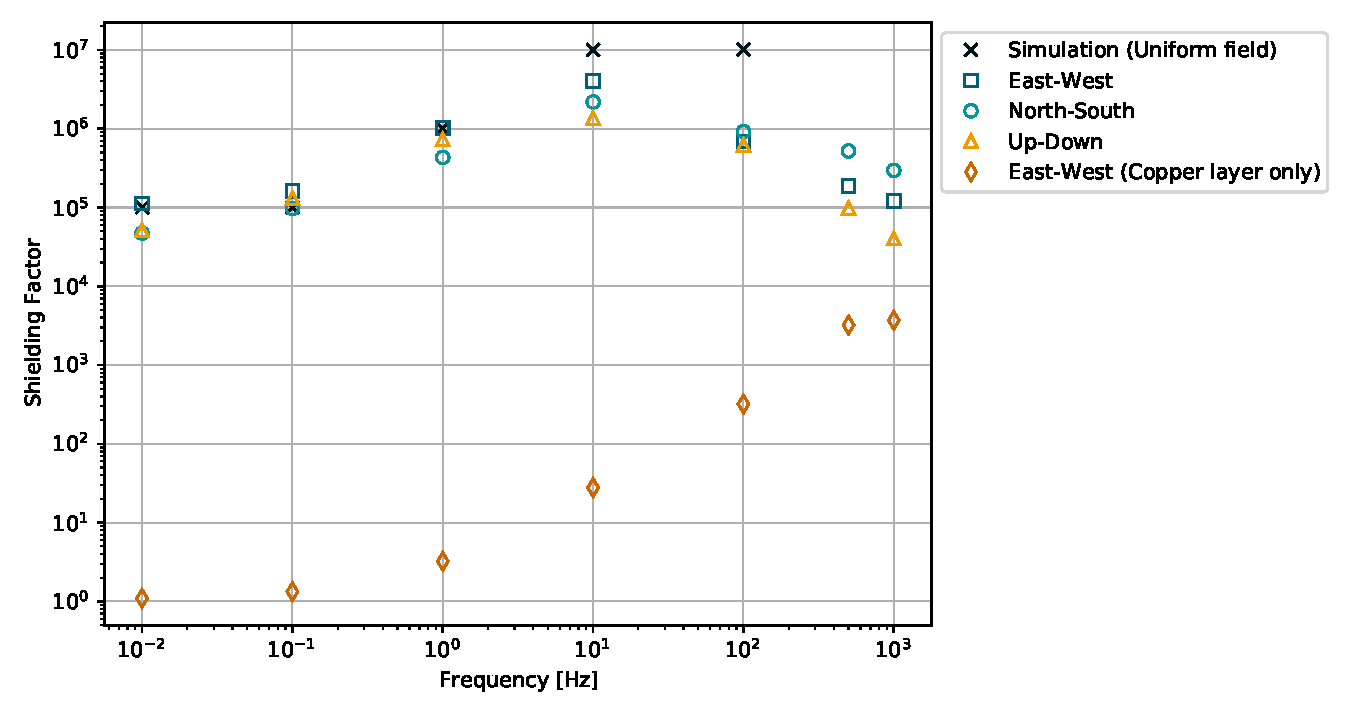
\includegraphics[width=\textwidth]{figures/chupp_msr_data.pdf}
    \caption
    {Calculated shielding factor of the LANL nEDM MSR (Tab.~\ref{tb:lanl_msr_shielding_factor}) for various orientations excitation signal directions of an infinitely sized coil. See Sec.~\ref{sec:MSR} for methodology.}
    \label{fig:MSR-shielding-factor}
\end{figure}

\begin{figure}
    \centering
    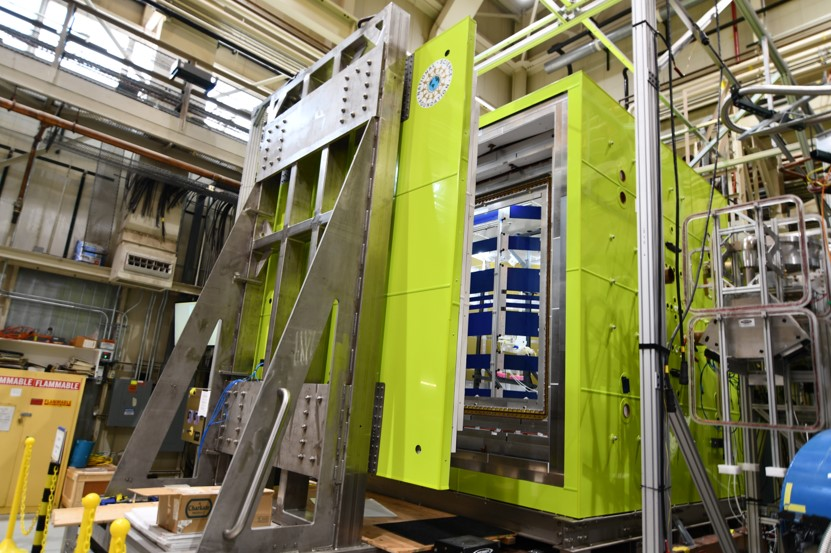
\includegraphics[width=0.9\textwidth]{figures/completed_msr.jpg}
    \caption
    {The LANL nEDM magnetically shielded room (Sec.~\ref{sec:MSR})}
    \label{fig:MSR}
\end{figure}

At LANL, a large magnetically shielded room (\acrshort*{msr}) (Fig.~\ref{fig:MSR}) is used for the attenuation of ambient external background magnetic fields. It has an overall shielding factor of $10^5$ for fields at frequency \qty{0.01}{\hertz} and a residual field of $<\qty{0.5}{nT}$.

The MSR consists of 4 Mumetal\textsuperscript{\textregistered} layers and one copper layer (Tab.~\ref{tb:lanl_msr_layers}). Mumetal\textsuperscript{\textregistered} is a magnetic shielding alloy ($\mu$-metal grade ASTM A753 Alloy 4, UNS N14080, 80NiFe) from the Magnetic Shield Corporation. The MSR utilizes a bolted construction to avoid welds that create magnetic domains. The frame of the MSR is stainless steel, which supports the load of the layers without deflection. The foundation consists of high density aggregate precast blocks, minimizing the transmission of ambient external vibrations.

For optimized shielding performance, the ferromagnetic layers are degaussed periodically. Degaussing is done by applying an alternating field with large amplitude, which drives the material to saturation, and then slowly decreasing the amplitude to zero. Each $\mu$-metal layer contains multiple L-shaped coil sets, activated sequentially, for complete degaussing coverage (see Fig.~\ref{fig:degaussing-paper-cube} for the layout of coils on the innermost layer).

\comment{Add LANL nEDM degaussing current amplitude}

Residual magnetic fields in the degaussed \acrshort*{msr} were measured with a low noise 3-axis Bartington fluxgate probe (Tab.~\ref{tb:lanl_msr_dc_residuals}). The fluxgate was mounted on a glass fiber structure, and was inserted through the large neutron guide access tubes of the MSR. At each position, a \qty{10}{\second} measurement per fluxgate axis was taken in addition to a corresponding measurement where the fluxgate was rotated by \qty{180}{\degree}.

The absolute magnetic field values for an axis ($i=x,y,z$) were then calculated using the relations
%
\begin{align}
    B_{i,\text{ un-rotated}}&=\text{offset}+B_{i}\\
    B_{i,\text{ rotated}}&=\text{offset}-B_{i}\\
    \text{offset}&= (B_{i,\text{ un-rotated}} + B_{i,\text{ rotated}})/2
\end{align}
%
From the offset-corrected field values, the measured gradient upper limit was found to be $\qty{0.51}{nT\per m}$.

Shielding factor was determined by using the LANL field cage (Sec.~\ref{sec:field-cage}) to provide excitation signals. The resulting amplitude was measured with a fluxgate at the center of the MSR both before the start of MSR construction and after construction was completed. The measured shielding factor was calculated from the ratio of the two amplitudes. Excitation signals of amplitude \qty{1}{\micro\tesla} were used for frequencies \qty{0.01}{\hertz} and \qty{0.1}{\hertz}, \qty{10}{\micro\tesla} for \qty{1}{\hertz}, and \qty{30}{\micro\tesla} for 10--\qty{1000}{\hertz}. 

To account for the finite size of the excitation coil and the iron floor of the experimental area, finite-element physics simulations in COMSOL were used to obtain a relation between the measured shielding factor and a calculated shielding factor with an ideal infinitely sized coil. This scaling was performed because the proximity of the field cage coils to the outer MSR layer resulted in localized saturation of the $\mu$-metal, artificially lowering the shielding factor. Shielding factors are shown in Fig.~\ref{fig:MSR-shielding-factor} and Tab~\ref{tb:lanl_msr_shielding_factor}. 

In the latter half of 2022, issues with the electrical contacts for the degaussing wires on the innermost MSR layer developed. This has delayed additional characterization of MSR performance.

\begin{table}
\centering
\caption{MSR layer composition}\label{tb:lanl_msr_layers}
\begin{tabular}{
    l
    c
    l
    S[table-format=1.2]
    c
    S[table-format=1.2]
    c
    S[table-format=1.2]
}
\toprule
Layer		& Thickness      & Material                        & \multicolumn{5}{c}{External side length}	\\
  &  {\scriptsize[mm]}    &  &  \multicolumn{5}{c}{$\text{\scriptsize [m}\scriptstyle\times \text{\scriptsize m}\scriptstyle\times\text{\scriptsize m]}$} \\
\midrule
1--outer	& 4  & Mumetal\textsuperscript{\textregistered}    & 3.5 & $\times$ & 3.5 & $\times$ & 3.5 \\
2	        & 3  & Mumetal\textsuperscript{\textregistered}    & 3.0 & $\times$ & 3.0 & $\times$ & 3.0 \\
3	        & 3  & Mumetal\textsuperscript{\textregistered}    & 2.6 & $\times$ & 2.6 & $\times$ & 2.6 \\
4	        & 8  & Copper                                      & 2.46 & $\times$ & 2.46 & $\times$ & 2.46 \\
5--inner	& 4  & Mumetal\textsuperscript{\textregistered}    & 2.39 & $\times$ & 2.39 & $\times$ & 2.39 \\
\bottomrule
\end{tabular}
% \end{table}
\vspace{\baselineskip}\vspace{\baselineskip}
% \begin{table}
% \centering
\caption{Residual DC fields in degaussed MSR. The measured gradient upper limit was found to be $\qty{0.51}{nT\per m}$}\label{tb:lanl_msr_dc_residuals}
\begin{tabular}{
    c
    S[table-format = 2.0]
    S[table-format = 2.0]
    S[table-format = 2.0]
    S[table-format = 1.2]
}
\toprule
Point		& $x$				& $y$				& $z$				& $|B|$	\\
{}    		& {\scriptsize(rel. to center)}	        & {\phantom{,,,}\scriptsize[cm]\phantom{,,,,}}       & {\scriptsize[cm]}		& {\scriptsize[nT]} 		\\
\midrule
1			& -40	            & -39	            & 23		        & 0.64\\
2			& 0	                & -39	            & 23	        	& 0.51\\
3			& 40                & -39	            & 23		        & 0.45\\
4			& -40	            & 39        		& -23	            & 0.52\\
5			& 0                 & 39        	    & -23	            & 0.41\\
6			& 40                & 39                & -23	            & 0.93\\
\bottomrule
\end{tabular}

% \end{table}
\vspace{\baselineskip}\vspace{\baselineskip}
% \begin{table}
% \centering
\caption{MSR shielding factors, measured and calculated (as per Sec.~\ref{sec:MSR})}\label{tb:lanl_msr_shielding_factor}
\begin{tabular}{
    c
    S[exponent-mode = scientific, table-format = 1.2e1]
    S[exponent-mode = scientific, table-format = 1.2e1]
}
\toprule
{Frequency}		& {Shielding factor}			& {Shielding factor}\\
{\scriptsize[Hz]}	& {\scriptsize(Measured)}	& {\scriptsize(corrected for geometry)} \\
\midrule
0.01    & 2.82e4    & 1.55e5 \\
0.1     & 4.55e4    & 2.50e5 \\
1       & 1.05e5    & 1.05e5 \\
10      & 7.72e4    & 4.25e5 \\
100     & 1.16e4    & 4.64e5 \\
\bottomrule
\end{tabular}

\end{table}


\begin{figure}
    \centering
    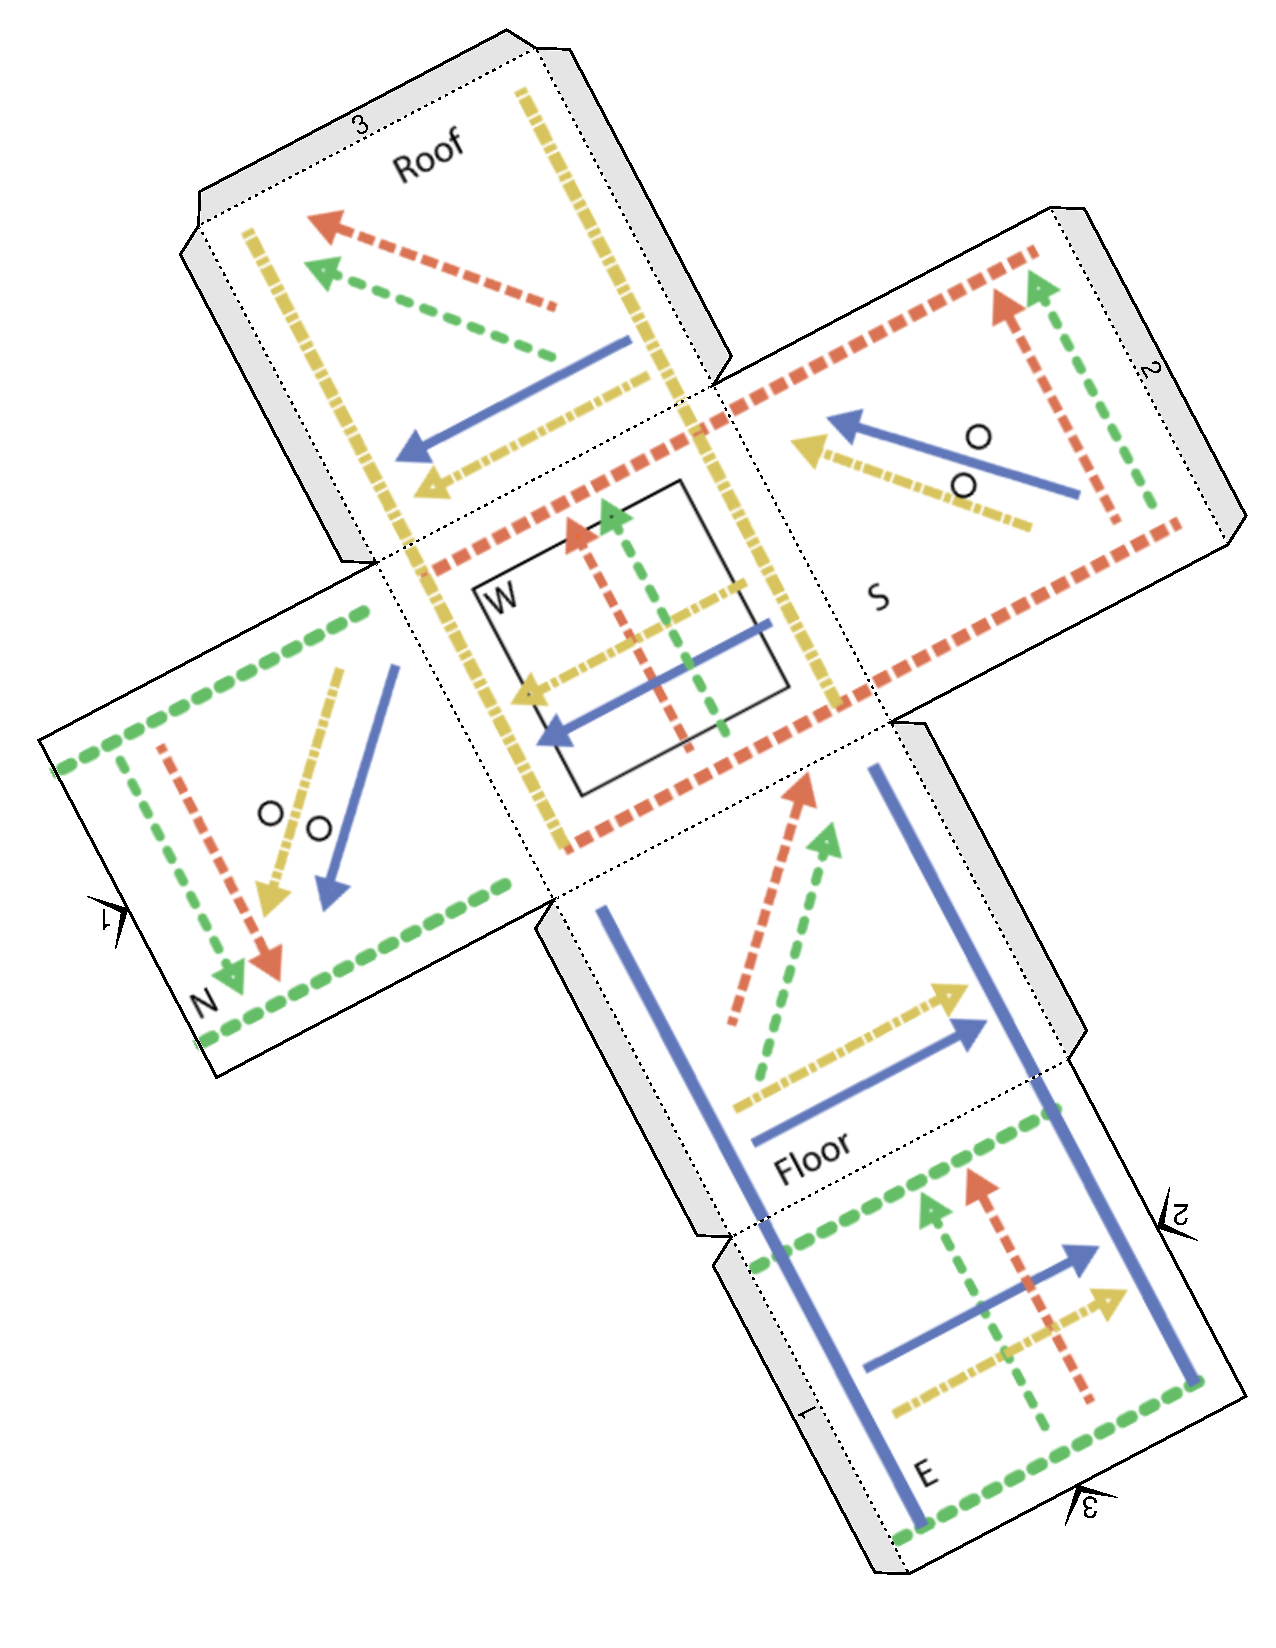
\includegraphics[width=\textwidth]{figures/L5-papercube.pdf}
    \caption
    {Simplified papercraft model of the four L-shaped degaussing coil sets on the innermost MSR layer and resulting flux contributions. Figure courtesy of Austin Reid.}
    \label{fig:degaussing-paper-cube}
\end{figure}

%%%%%%%%%%%%%%%%%%%%%%%%%%%%%%%%%%%%%%%%%

\section{External field compensation coils}\label{sec:field-cage}

%%%%%%%%%%%%%%%%%%%%%%%%%%%%%%%%%%%%%%%%%

\begin{figure}
\centering
\begin{minipage}{.5\textwidth}
    \centering
    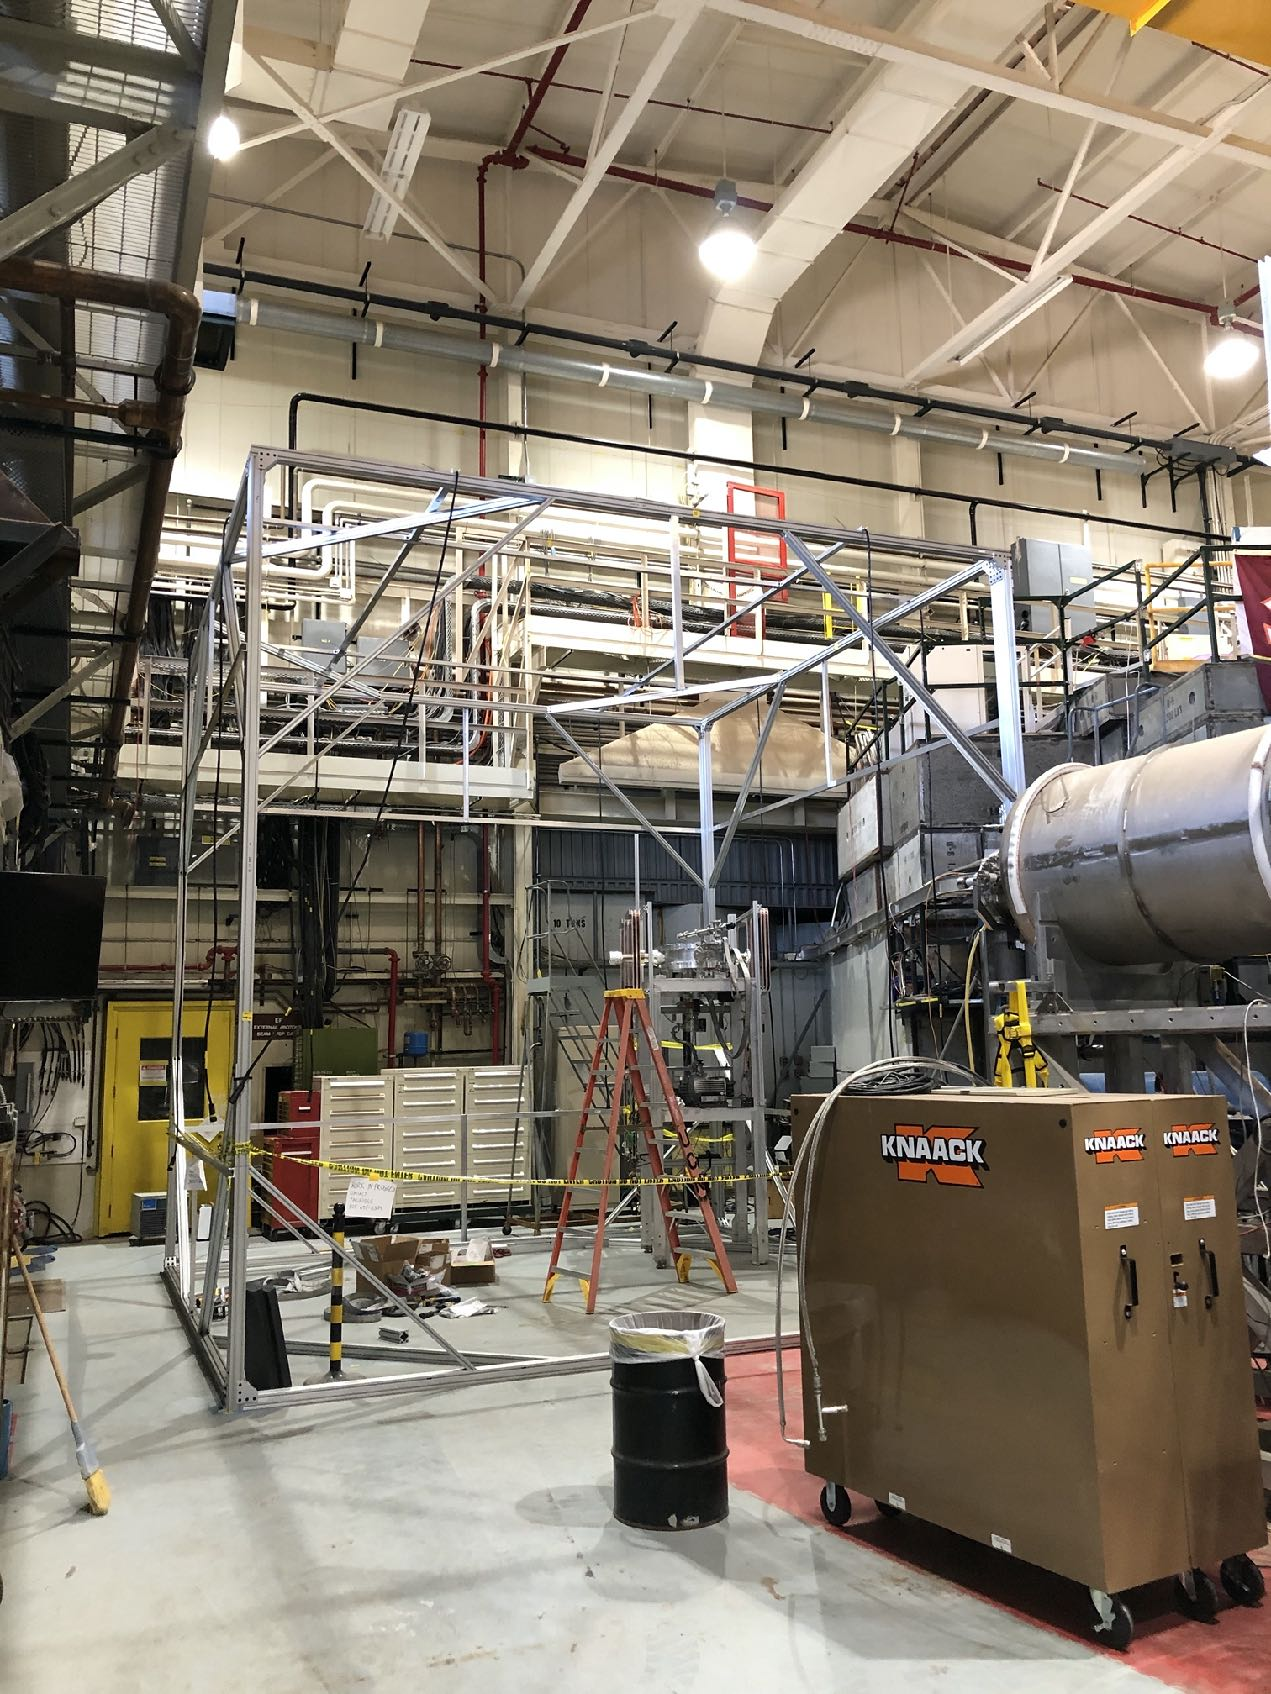
\includegraphics[height=4in]{figures/field_cage_no_msr.jpg}
    \caption
    {LANL nEDM field cage (Sec.~\ref{sec:field-cage})}
    \label{fig:lanl-field-cage}
\end{minipage}%
\begin{minipage}{.5\textwidth}
    \centering
    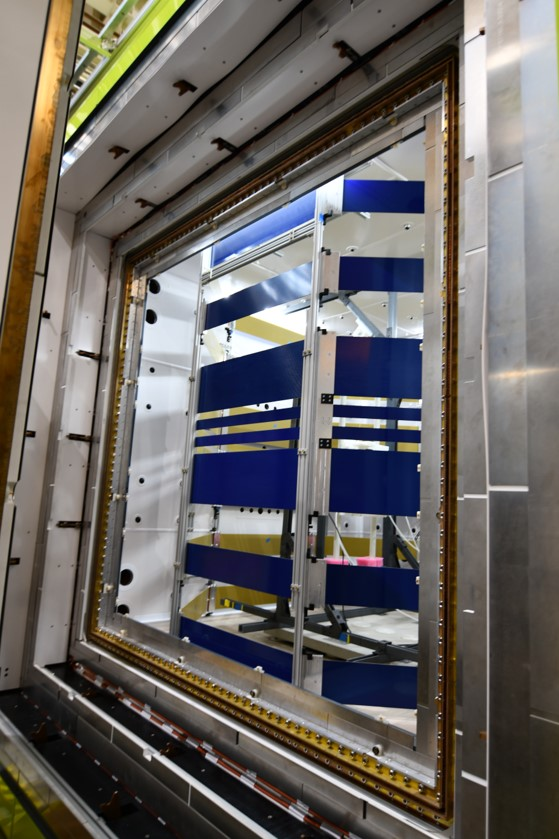
\includegraphics[height=4in]{figures/b0_zoom_in.jpg}
    \caption
    {Installed $B_0$ coil}
    \label{fig:lanl-b0-coil}
\end{minipage}
\end{figure}

\begin{figure}
\centering
\begin{minipage}{.5\textwidth}
    \centering
    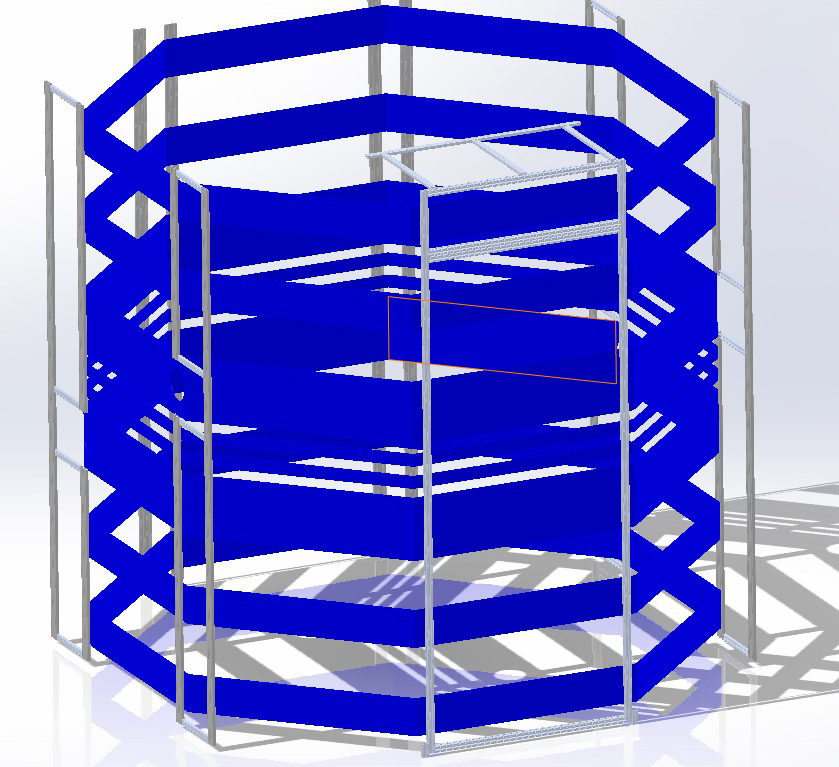
\includegraphics[width=0.9\textwidth]{figures/B0-model.png}
    \caption
    {Model of $B_0$ coil (Sec.~\ref{sec:B0_coil})}
    \label{fig:b0-coil-model}
\end{minipage}%
\begin{minipage}{.5\textwidth}
    \centering
    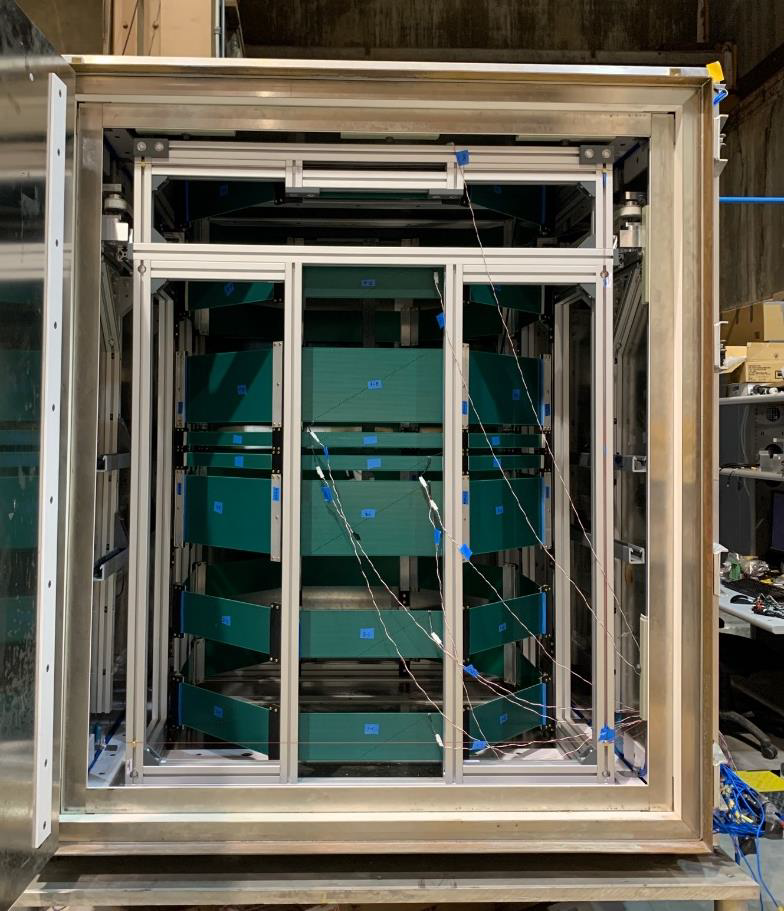
\includegraphics[width=0.9\textwidth]{figures/half-scale-B0.png}
    \caption
    {Half-scale $B_0$ coil prototype in the 2-layer MSR}
    \label{fig:b0-half-scale}
\end{minipage}
\end{figure}

The external compensation coils, or ``field cage,'' (Fig.~\ref{fig:lanl-field-cage}) provide up to \qty{32}{\micro\tesla} to offset ambient fields. The field cage was used for the determination of the MSR shielding factor (Sec.~\ref{sec:MSR}). In the eventual LANL nEDM experiment a PID controller will enable active reduction of external field drifts.

%%%%%%%%%%%%%%%%%%%%%%%%%%%%%%%%%%%%%%%%%

\section{
    \texorpdfstring{$B_0$ coil}
                {B0 coil}\label{sec:B0_coil}
}

%%%%%%%%%%%%%%%%%%%%%%%%%%%%%%%%%%%%%%%%%

The LANL nEDM $B_0$ holding coil is a split solenoid consisting of 8 octagonal sections (Figs.~\ref{fig:lanl-b0-coil}, \ref{fig:b0-coil-model}). Each section comprises of printed circuit boards (PCBs) and custom 3D-printed connections. The gaps between each section serve the purpose of accomodating neutron guides, comagnetometer lasers, \acrshort*{hv} cables, vacuum pump lines, etc. The modularized $B_0$ design allows removal of PCB segments from the octagon for access to the experiment. The $B_0$ coil is coupled to the innermost layer of the MSR for purposes of flux return. 

The uniformity of the field is adjusted by tuning the currents in each section of the coil. While initial measurements with fluxgates indicate that the vertical gradient meets specifications $(\partial B_0/\partial dz < \qty{1}{nT \per m})$, further $B_0$ field uniformity measurements have been delayed due to the issue with the degaussing loop contacts (Sec.~\ref{sec:MSR}).

The $B_0$ coil has undergone several prototyping stages. An initial prototype was constructed for the Ramsey demonstration in 2017 (Chap.~\ref{chap:lanl_ramsey_demonstration}). A half scale prototype was also tested at LANL in a 2-layer MSR (Fig.~\ref{fig:b0-half-scale}).

%%%%%%%%%%%%%%%%%%%%%%%%%%%%%%%%%%%%%%%%%

\section{Transport coils}

%%%%%%%%%%%%%%%%%%%%%%%%%%%%%%%%%%%%%%%%%

\begin{figure}
\centering
\begin{minipage}{.5\textwidth}
    \centering
    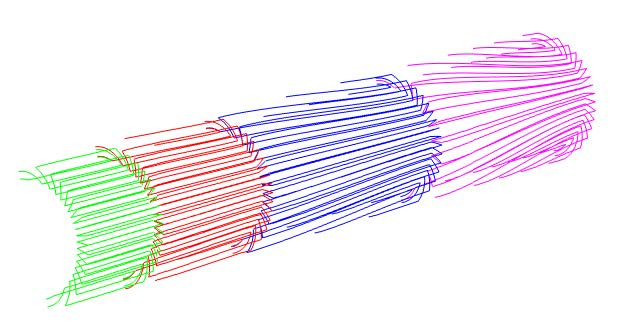
\includegraphics[width=\textwidth]{figures/transport_coil_mockup.jpg}
\end{minipage}%
\begin{minipage}{.5\textwidth}
    \centering
    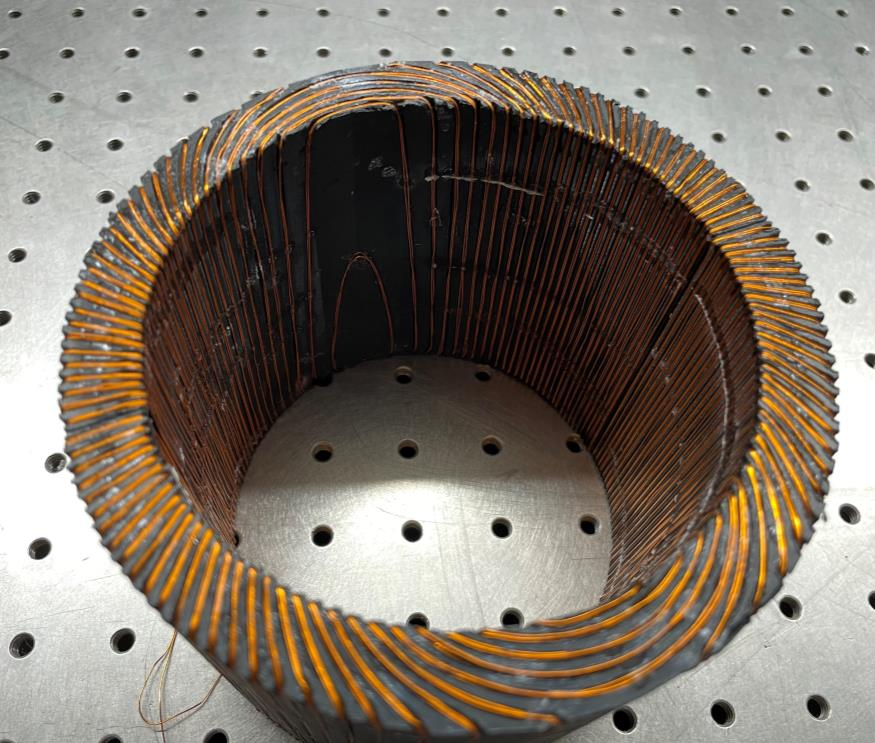
\includegraphics[width=\textwidth]{figures/transport_coil.jpg}
\end{minipage}
    \caption
    {Double layer $\cos\theta$ coil for transport from Earth's field to the $B_0$ field in the MSR. Figure provided by Piya Amara Palamure.}
    \label{fig:transport-coils}
\end{figure}

A set of spin transport coils are used to adiabatically transport UCNs from the ambient external magnetic field ($\sim\qty{20}{\micro T}$) through multiple layers of MSR shielding to the $B_0$ holding field ($\sim\qty{1}{\micro T}$. The design is a modified double layer $\cos\theta$ coil, which provides self-shielding to limit the magnetization of surrounding MuMetal. The innermost transport coil segment interfaces directly with a $B_0$ PCB panel with a hole to avoid possible field zeros that would depolarize \ucn. 

%%%%%%%%%%%%%%%%%%%%%%%%%%%%%%%%%%%%%%%%%

\section{Magnetic Impurity Scanner}\label{sec:magnetic_impurity_scanner}

%%%%%%%%%%%%%%%%%%%%%%%%%%%%%%%%%%%%%%%%%

\begin{figure}
    \centering
    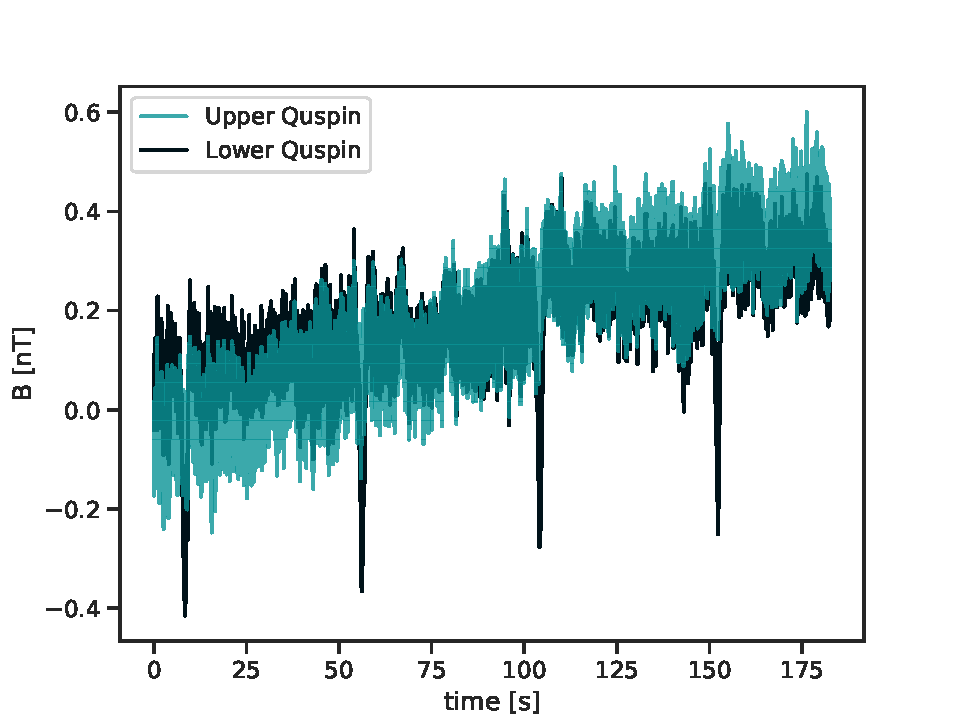
\includegraphics[width=0.7\textwidth]{figures/magnetic_contamination_example.pdf}
    \caption
      {Example of magnetic impurities on a rejected experimental component found by the scanning setup in Sec.~\ref{sec:magnetic_impurity_scanner}. The component is mounted on a slowly-moving turntable, and the periodic spike is correlated to when the part passes beneath the magnetometers. The QuSpin magnetometers are in a gradiometer configuration, such that there is a vertical separation between sensors of \qty{0.75}{in}.}
    \label{fig:magnetic_contamination_example}
\end{figure}

\begin{figure}
    \centering
    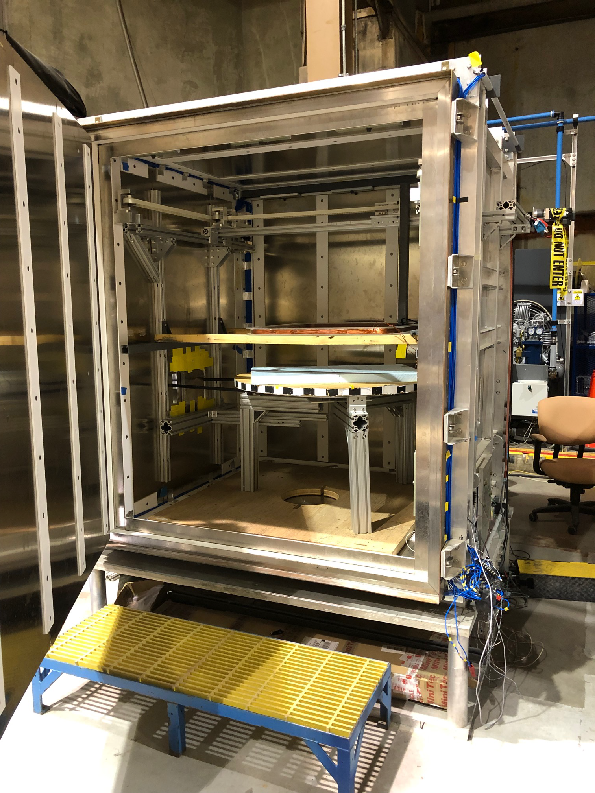
\includegraphics[height=3.5in]{figures/magnetic_impurity_scanner.png}
    \caption
      {Magnetic impurity scanner at LANL. In a 2-layer MSR, a nonmagnetic turntable passes parts beneath two QuSpin Total-Field Magnetometers.}
    \label{fig:magnetic_impurity_scanner}
\end{figure}

Localized magnetic sources (``contamination'') embedded within the precession cell and other experimental components create volume-averaged gradients that would lead to a false EDM signal. Any component installed within the MSR was subject to a scanning procedure to screen for contamination. Parts were mounted on a nonmagnetic turntable located in a 2-layer MSR at LANL (Fig~\ref{fig:magnetic_impurity_scanner}). The turntable was actuated by a belt system connecting to a motor outside the MSR. The parts were slowly passed beneath two Rb SERF magnetometers in a gradiometer configuration, where the vertical separation between sensors was \qty{0.75}{in}. Components with nonzero magnetic signal were subjected to additional cleaning procedures, and, failing that, were rejected from use within the MSR.

The current magnetic impurity scanner can detect contamination on the order $\sim\qty{0.1}{nT}$ (Fig.~\ref{fig:magnetic_contamination_example}). The magnetometers are QuSpin Total-Field Magnetometers, which have a sensitivity of $<\qty{1}{pT\per\sqrt{Hz}}$ in the 0.1--\qty{100}{\hertz} range. The use of these magnetometers required a large helmholtz coil installed around the turntable to provide a small bias field. With improvements to the quality of the magnetic environment (e.g. extra shielding, reduced ambient magnetic noise) it will be possible to switch to QuSpin Zero-Field Magnetometers, which have a sensitivity $<\qty{1}{pT\per\sqrt{Hz}}$ for 1--\qty{100}{\hertz}.

Appendix~\ref{appx:magnetic_contamination} demonstrates the characterization process for a source of magnetic contamination found on a rejected component.

%%%%%%%%%%%%%%%%%%%%%%%%%%%%%%%%%%%%%%%%%

\section{Polarizing magnet}\label{sec:PM_description}

%%%%%%%%%%%%%%%%%%%%%%%%%%%%%%%%%%%%%%%%%

A \qty{5}{\tesla}, horizontal warm bore, superconducting magnet by American Magnetics Inc. is used as a polarizing magnet (\acrshort*{pm}). The PM field filters UCN spins, acting as a potential barrier that rejects low-field seeking UCN below \qty{300}{\nano\eV} and a potential well that passes high-field seeking UCN (Sec.~\ref{sec:ucn_polarizers}). 

A \qty{0.1}{\milli\meter} thick Al97 Mg3 alloy foil (similar in tensile strength to 6061-T6), termed the ``PM window," is located in the beamline at the center of the PM field region. This is used to separate the UCN source vacuum from the measurement apparatus vacuum, as the source vacuum can be routinely filled with D$_2$ gas (e.g. while D$_2$ is being drawn from a storage tank to be frozen or while SD$_2$ is being reconditioned). The magnetic potential of the PM overwhelms the neutron optical potential of the window (\qty{54}{\nano\eV} \cite{golubUCN}). The effect of the window on the transmission of UCN is discussed in detail in Sec.~\ref{sec:analysis}.

%%%%%%%%%%%%%%%%%%%%%%%%%%%%%%%%%%%%%%%%%

\section{Spin flipper and analyzers}\label{sec:spin_flipper_analyzer}

%%%%%%%%%%%%%%%%%%%%%%%%%%%%%%%%%%%%%%%%%

Neutron spin analyzers in the LANL nEDM are 10 layer polarizers made of iron and silicon located immediately above neutron detectors (see Ref.~\cite{ThorstenThesis} for layer structure details). When magnetized with a ($\sim \qty{10}{mT}$) field from permanent magnets, the multi-layer polarizer preferentially transmits high-field seeking UCN and rejects low-field seeking UCN with an analyzing power of $99.3^{+0.7}_{-2.4}\%$~\cite{ThorstenThesis}.

Note that it is not clear if the neutron energy spectrum under which Ref.~\cite{ThorstenThesis} is consistent with the LANL nEDM neutron spectrum. Reference~\cite{afach_device_2015} quotes an analyzing power of 95\% for a different but similar analyzing foil for an energy range of 90~neV to 330~neV, which includes the energy range of the UCN at the analyzing foil for the experiment reported in Sec.~\ref{sec:analysis}. Additional analyzing power characterization measurements are planned.

Additionally, an adiabatic fast passage (\acrshort{afp}) spin flipper coil, located upstream of the spin analyzer, is used to provide the option of spin flipping UCN (Sec.~\ref{sec:afp}). A schematic of the analyzer system is illustrated in Fig.~\ref{fig:SpinAnalyzer}.

\begin{figure}
    \centering
    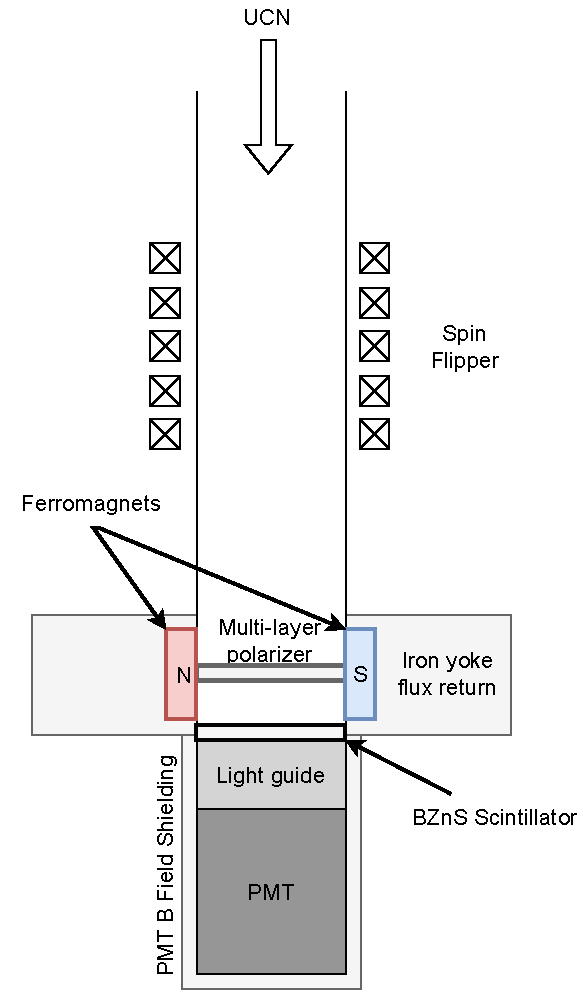
\includegraphics[width=5cm]{spinAnalyzer.pdf}
    \caption{Schematic of the adiabatic fast passage (\acrshort{afp}) spin flipper, spin analyzer, and UCN drop detector}
    \label{fig:SpinAnalyzer}
\end{figure}

%%%%%%%%%%%%%%%%%%%%%%%%%%%%%%%%%%%%%%%%%

\section{UCN detectors}\label{sec:ucn_detectors}

%%%%%%%%%%%%%%%%%%%%%%%%%%%%%%%%%%%%%%%%%

We use $\ce{^{10}B}$ coated ZnS:Ag scintillator films for UCN detection \cite{jeph_b10_2011}. UCN are captured on the top layer of $\ce{^{10}B}$, and reaction products ($^4$He and/or $^7$Li) from the $\ce{^{10}B}(\text{n},\alpha)^7\text{Li}$ neutron capture reaction are detected in the ZnS:Ag layer. The resulting scintillation light is then amplified by a photomultiplier tube (\acrshort*{pmt}) or silicon photomultiplier (\acrshort*{sipm}).

%%%%%%%%%%%%%%%%%%%%%%%%%%%%%%%%%%%%%%%%%

\section{UCN switchers}\label{sec:lanl_switchers}

%%%%%%%%%%%%%%%%%%%%%%%%%%%%%%%%%%%%%%%%%

\begin{figure}
    \centering
    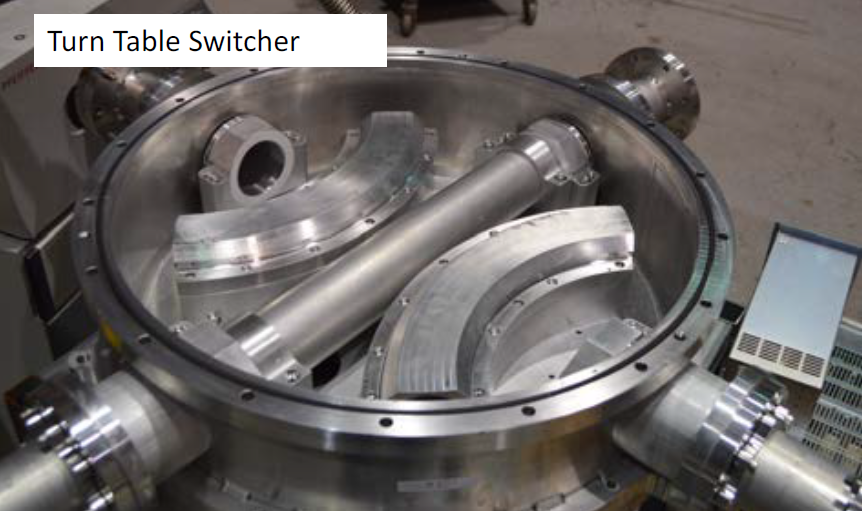
\includegraphics[width=7cm]{NewSwitcher.png}
    \hspace{1em}
    % 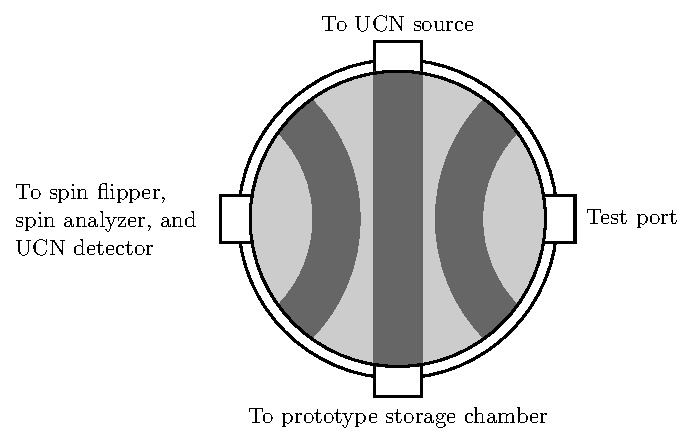
\includegraphics[width=0.5\textwidth]{North_Beamline_Switcher_Figure.pdf}
    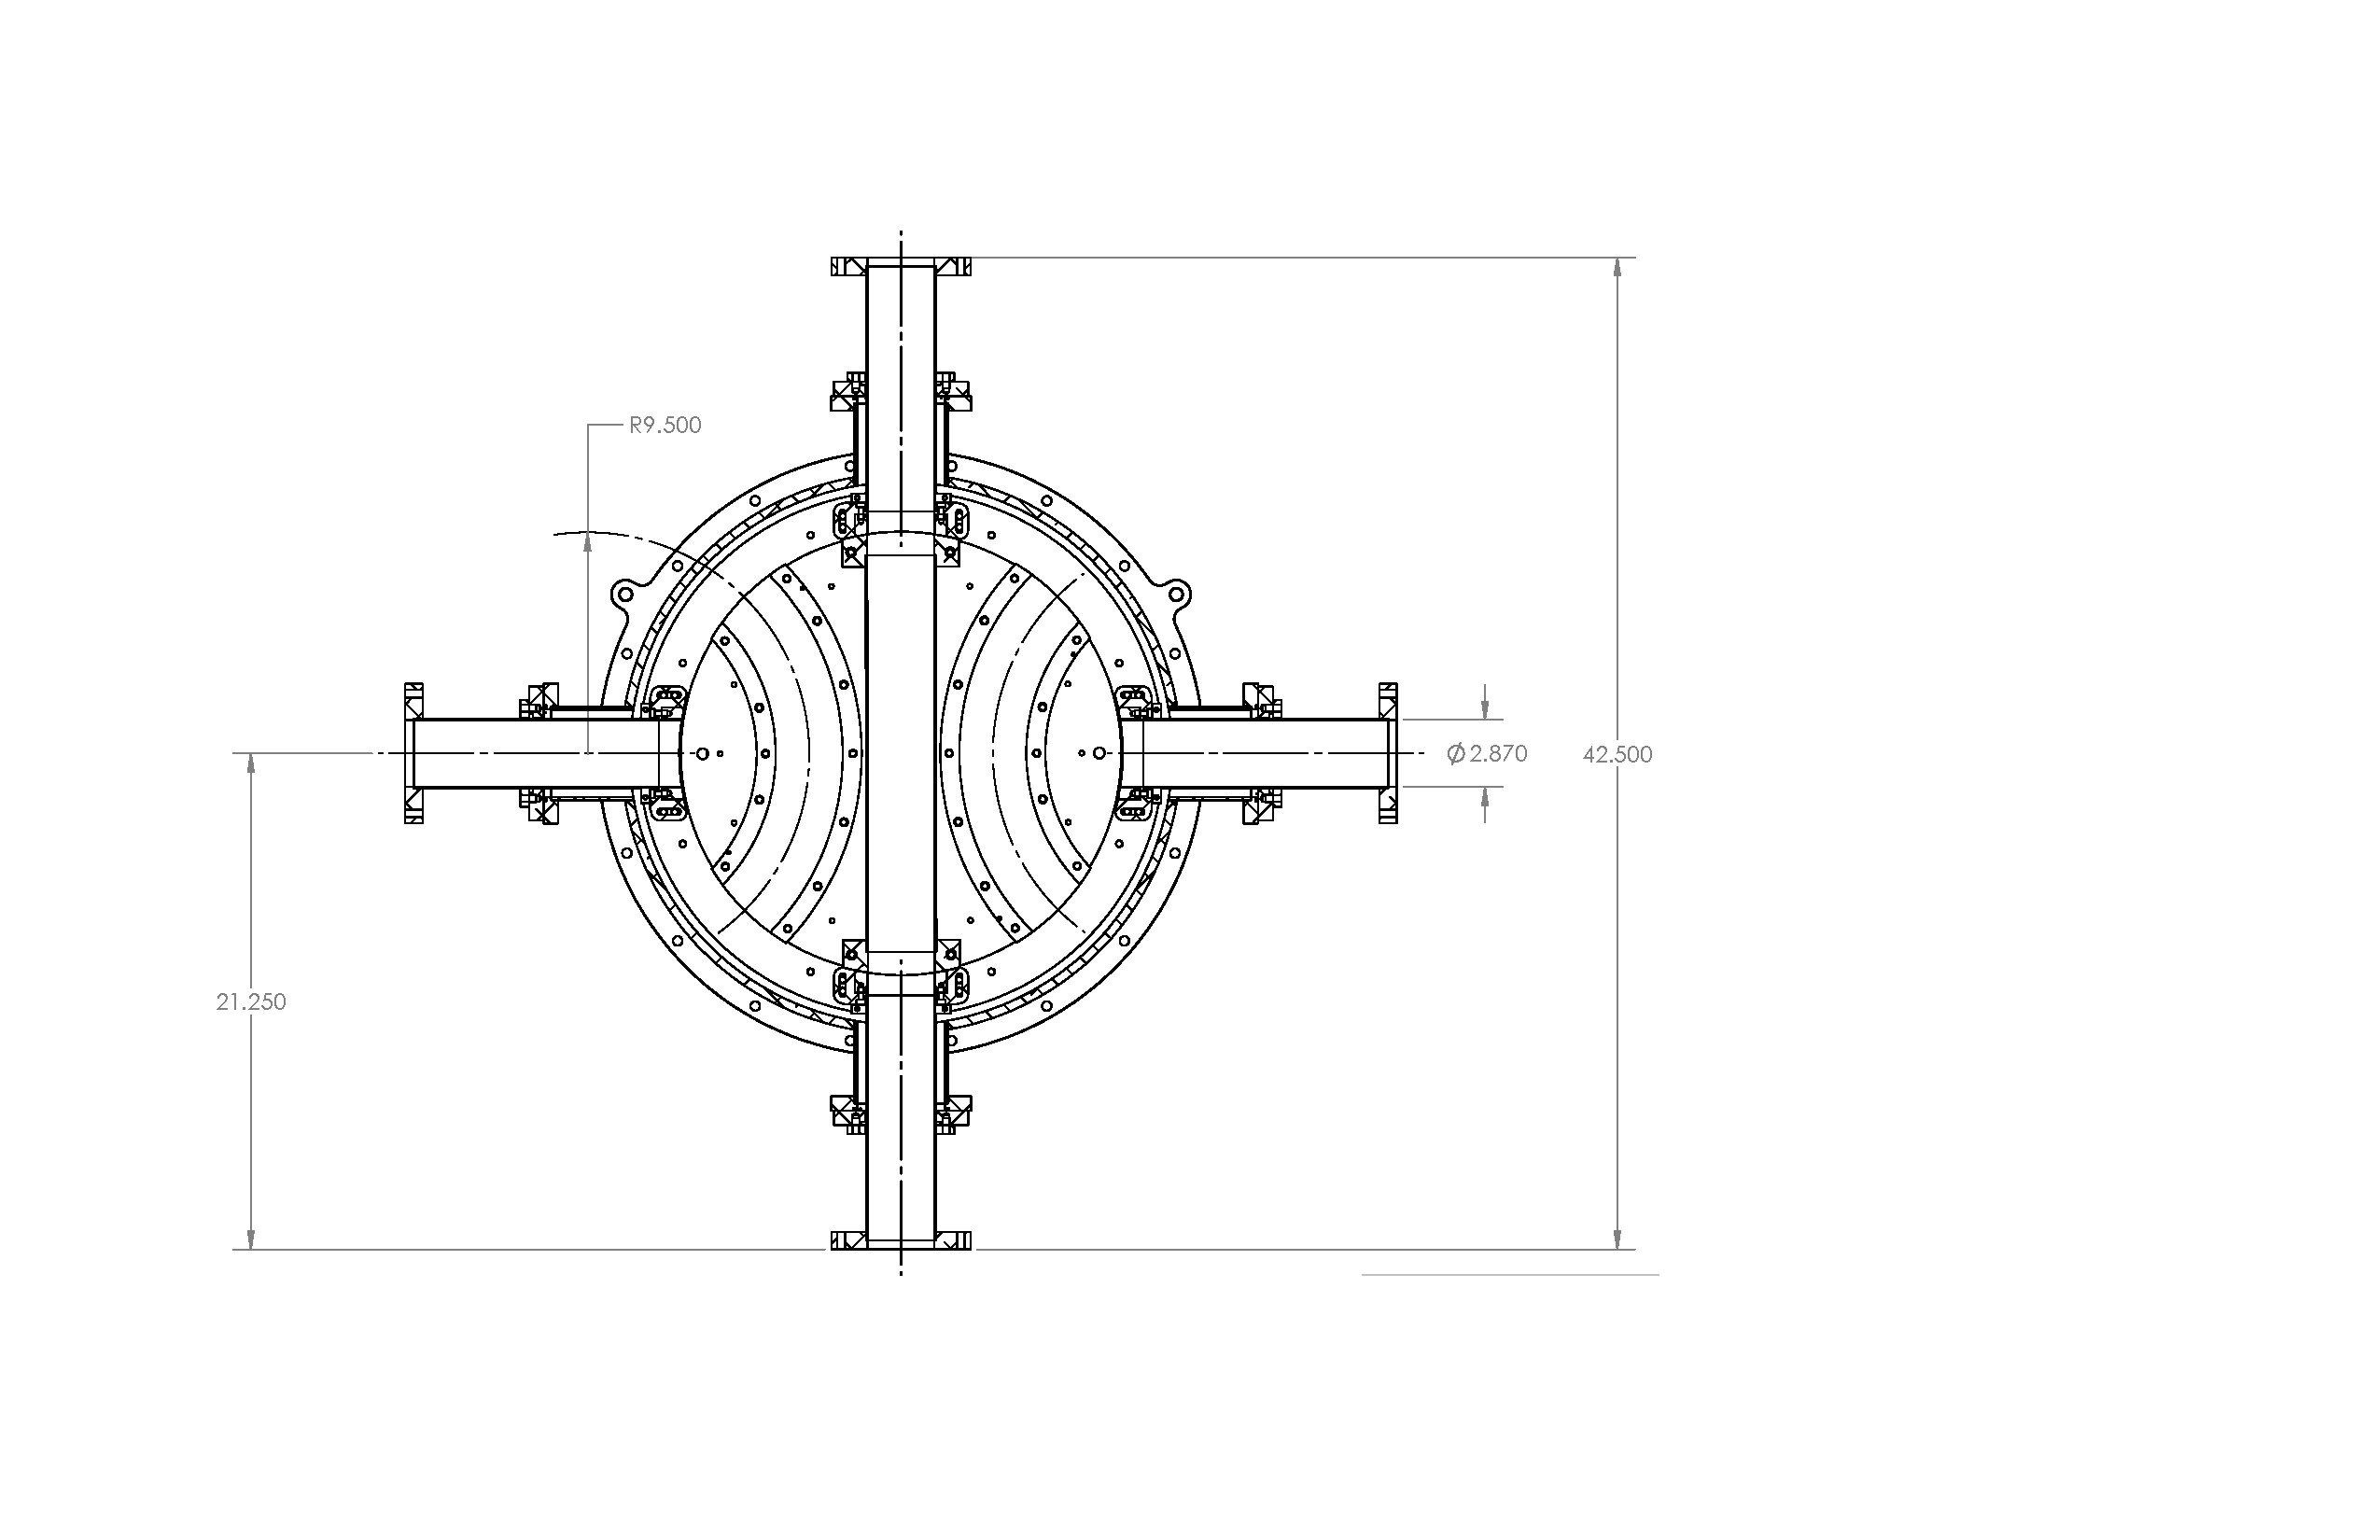
\includegraphics[width=0.5\textwidth]{figures/switcher_schematic.pdf}
    \caption[Photograph and schematic of rotary switcher]{Left: A photograph of the switcher. Right: Top-down schematic of the rotary switcher}\label{fig:NewSwitcher}
\end{figure}

The LANL nEDM uses two switchers for neutron transport, one per precession cell. Each switcher has a cylindrical housing and four evenly spaced guide ports. These guide ports can be connected internally by either a straight guide section or \ang{90} bend sections. The internal guide sections are mounted on a rotating turntable and actuated by a Parker CM232DX servo-motor. The internal guide surfaces are coated with NiP and the interface of guide ports to the turntable-mounted guide sections is lined with PTFE to allow for minimal gaps between guide segments (see Tab.~\ref{tb:optical_potentials} for optical potentials). An image of the ``rotary switcher'' as well as a schematic of the guide segments within it are shown in Fig.~\ref{fig:NewSwitcher}. A study comparing the performance of this switcher design to a different prototype is performed in Chap.~\ref{chap:north_beamline_paper}.

%%%%%%%%%%%%%%%%%%%%%%%%%%%%%%%%%%%%%%%%%

\section{Precession cells}\label{sec:precession_cells}

%%%%%%%%%%%%%%%%%%%%%%%%%%%%%%%%%%%%%%%%%

\begin{figure}
    \centering
    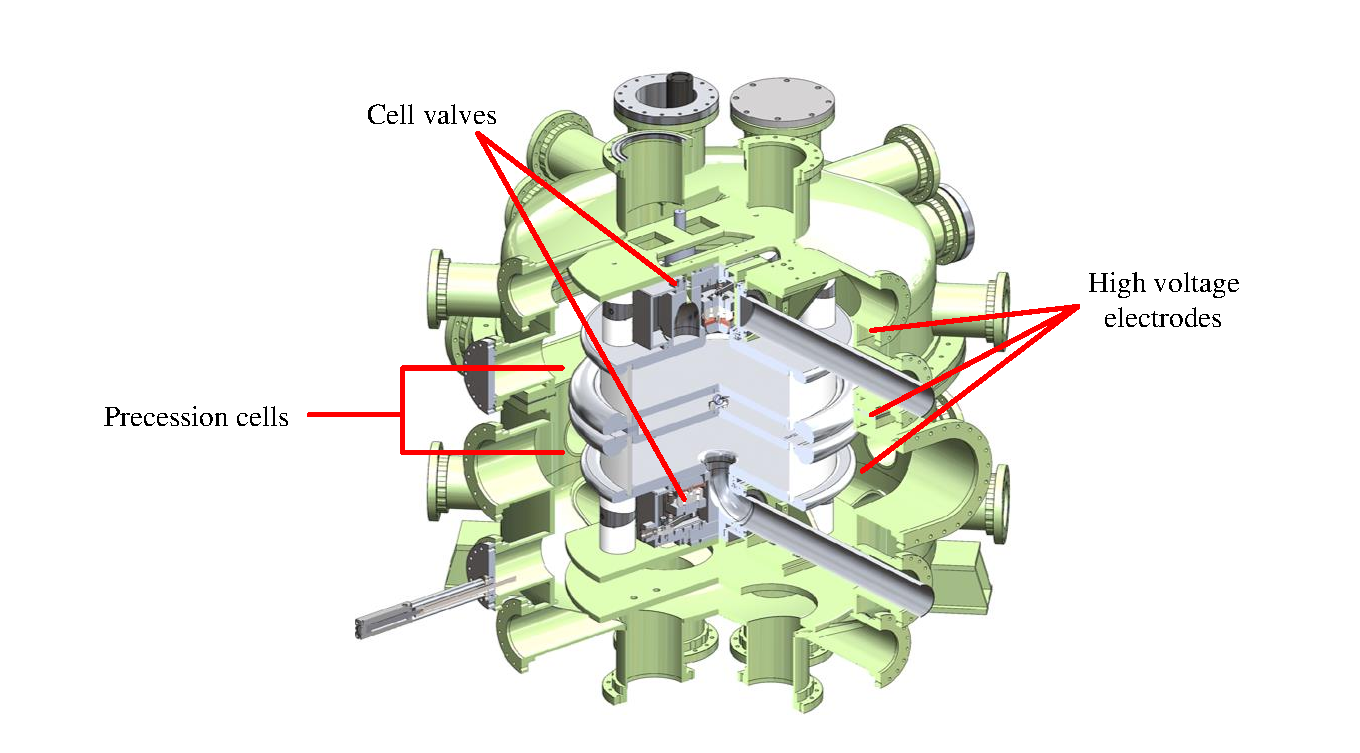
\includegraphics[width=0.85\textwidth]{figures/vacuum_chamber_cross.pdf}
    \caption
    {Cross section of the central apparatus, including the vacuum chamber, cell valves, HV electrodes, and precession cells}
    \label{fig:central_app_cross}
\end{figure}

\begin{figure}
\centering
\begin{minipage}{.5\textwidth}
    \centering
    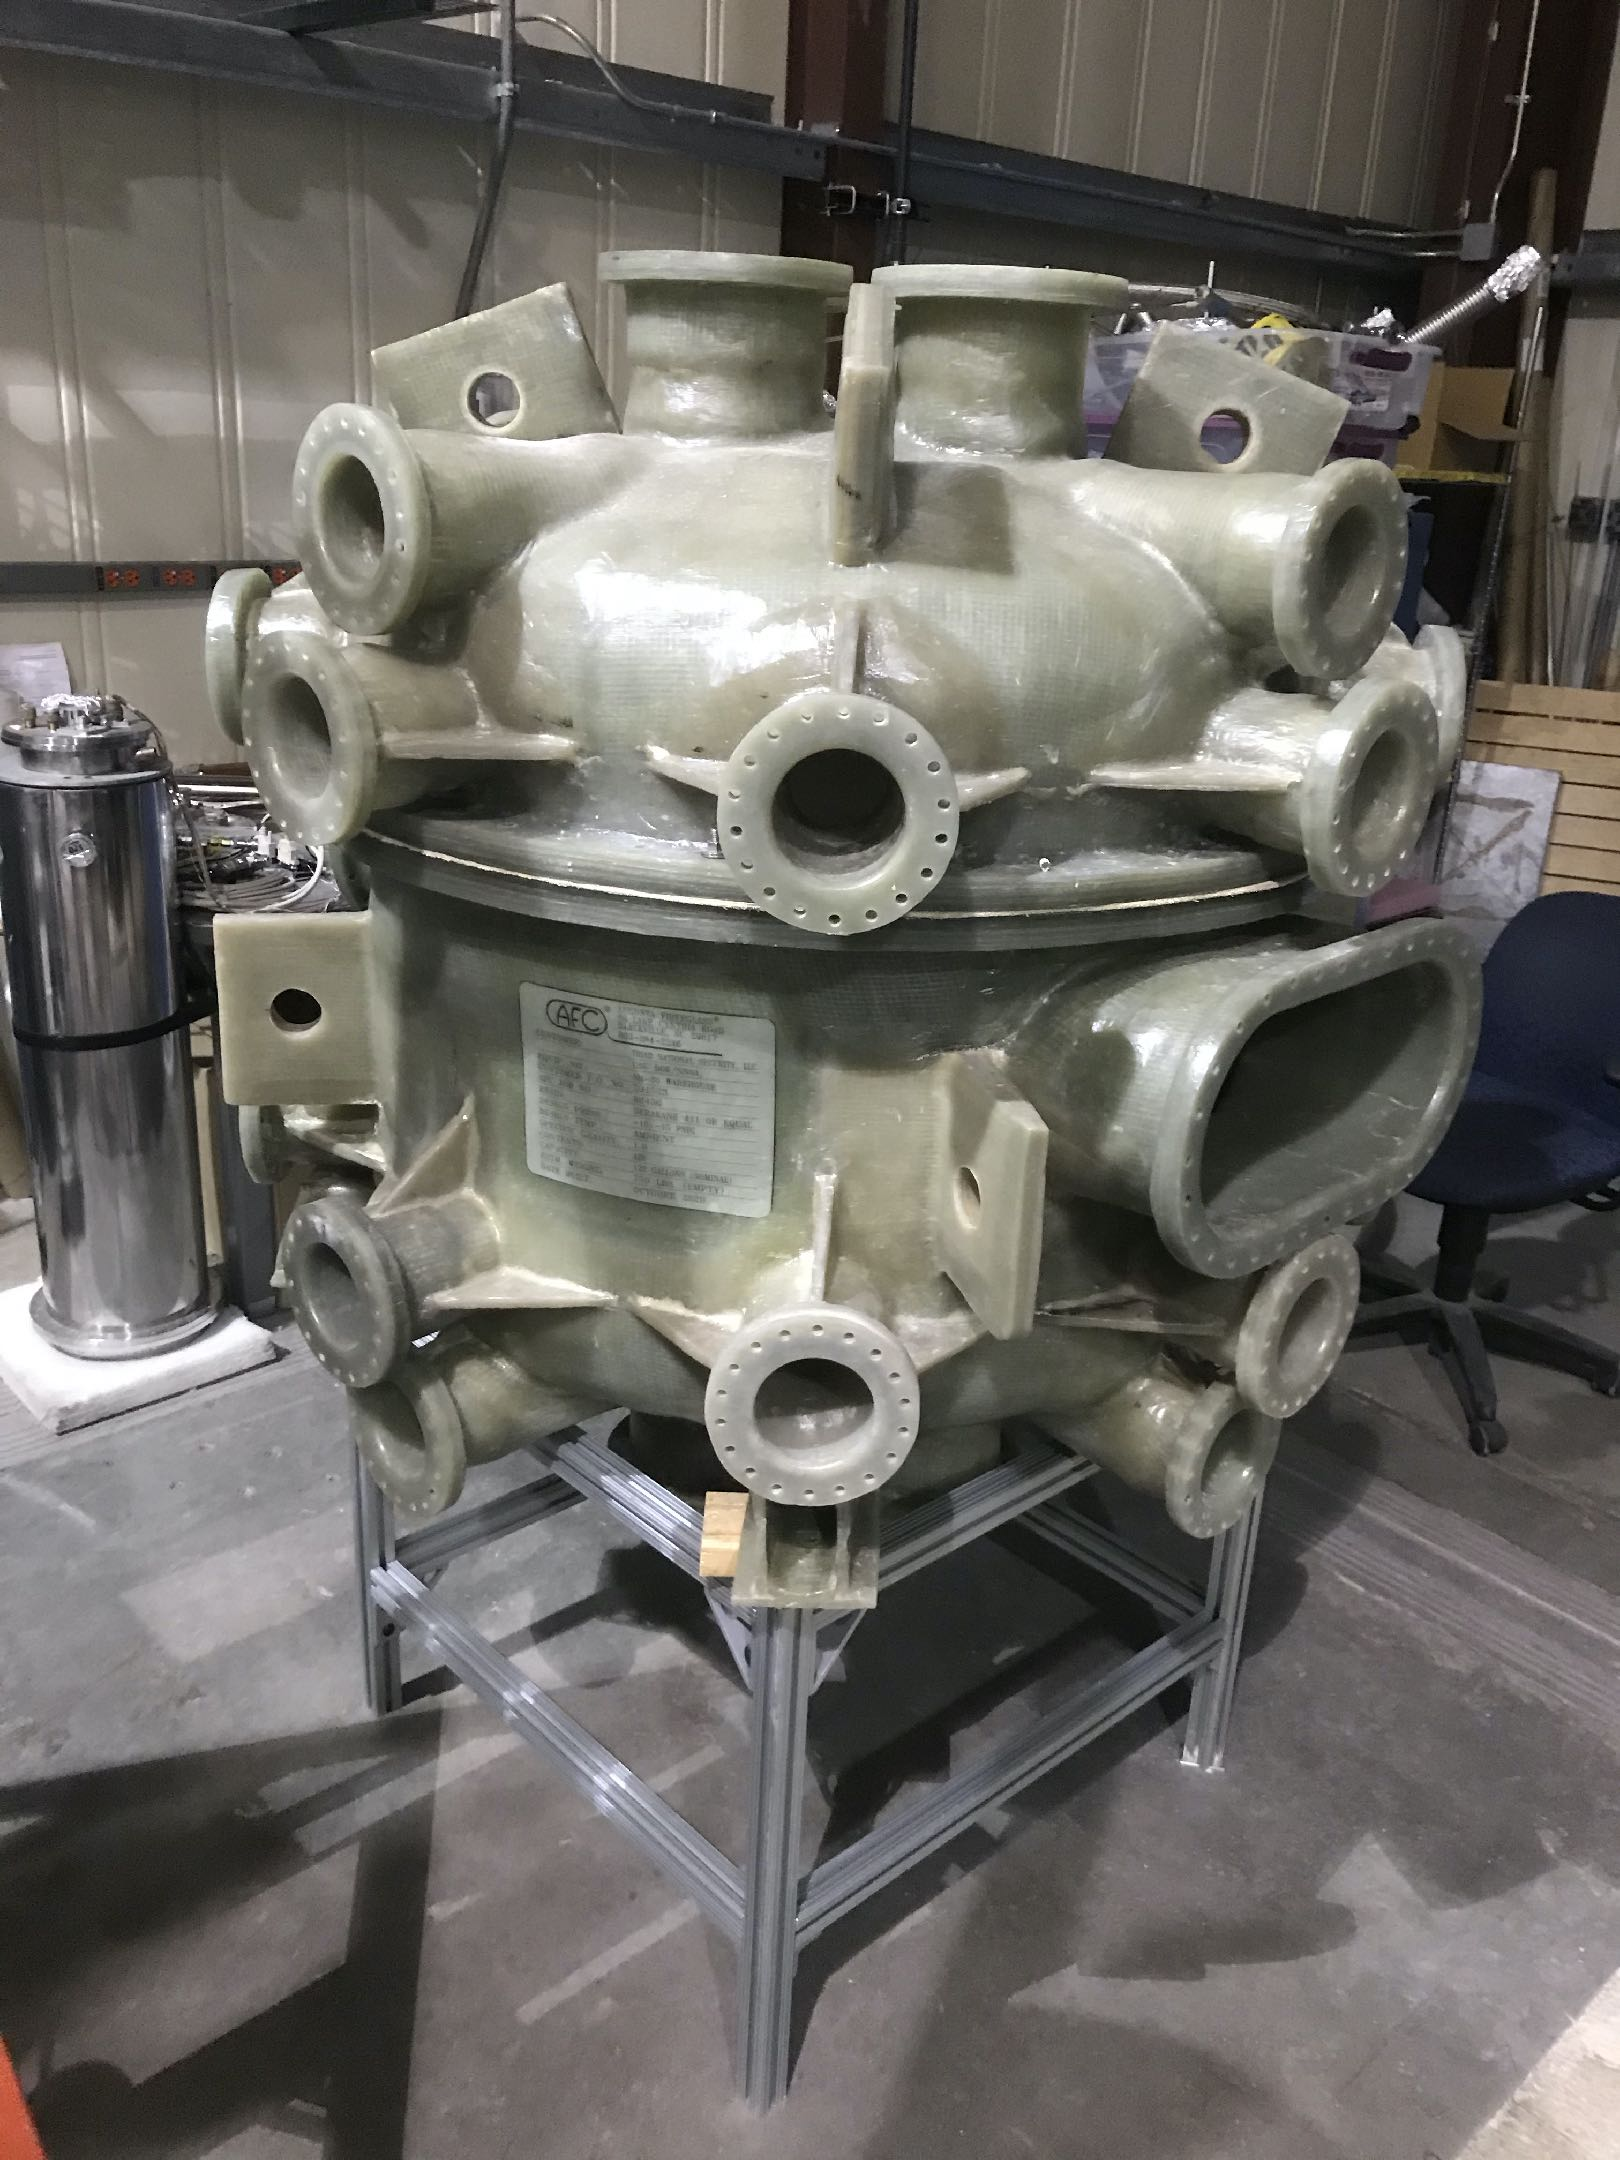
\includegraphics[height=4in]{figures/vacuum_chamber.jpg}
    \caption{Fiberglass vacuum chamber}
    \label{fig:vacuum_chamber}
\end{minipage}%
\begin{minipage}{.5\textwidth}
    \centering
    \includegraphics[width=4in,angle=90]{figures/cell_valve.jpg}
    \caption
    {Cell valve}
    \label{fig:cell_valve}
\end{minipage}
\end{figure}

The two precession cells, responsible for storage of polarized \ucn and \hg atoms, are formed by parallel-plate electrodes sandwiching a poly(methyl methacrylate) (\acrshort*{pmma}) insulator. The PMMA cell walls are coated with deuterated polystyrene (\acrshort*{dps}) (Sec.~\ref{sec:dPS_coating}). The chambers are designed with the ground electrodes on the top and bottom of the apparatus, and the HV electrodes in the middle (connected to a HV feedthrough). This enables simultaneous measurement of $\vv{B}_0\uparrow\uparrow\vv{E}$ and $\vv{B}_0\uparrow\downarrow\vv{E}$ configurations, cancellation of temporal field drifts to first order, and roughly doubles neutron counting statistics per cycle (see Sec.~\ref{sec:north_beamline_discussion}).

Each precession chamber has an inner diameter of \qty{50}{cm} and a height of \qty{10}{cm}. The final nEDM experiment will use electrodes coated in diamond-like carbon (\acrshort*{dlc}), though the measurements presented in this dissertation primarily use \acrshort{nip}-coated prototype electrodes (see discussion in Sec.~\ref{subsec:holdingTimeMeasurement}).

The precession cells are enclosed by a custom fiberglass vacuum chamberfrom Augusta Fiberglass Coating Inc. (Fig.~\ref{fig:vacuum_chamber}). The material was selected to avoid attenuation of the RF $\pi/2$ pulse.

The cell valves (Fig.~\ref{fig:cell_valve}) consist of Nickel Molybdenum (\acrshort*{nimo}) coated parts and NiP-coated guide segments mounted on G-10 fiberglass plates. The actuation system is hydraulic and routed outside the MSR to a STM23Q motor that controls a piston. This prevents the generation of undesired magnetic fields during cell valve actuation. The moving faces of the cell valve are sealed with PTFE-coated o-rings for maintenance of a separate vacuum from the vacuum chamber.

%%%%%%%%%%%%%%%%%%%%%%%%%%%%%%%%%%%%%%%%%

\subsection{Precession cell dPS coating}\label{sec:dPS_coating}

%%%%%%%%%%%%%%%%%%%%%%%%%%%%%%%%%%%%%%%%%

\begin{figure}
\centering
%subfigure width gets "multiplied" by includegraphics width
\begin{subfigure}{.5\textwidth} 
  \centering
  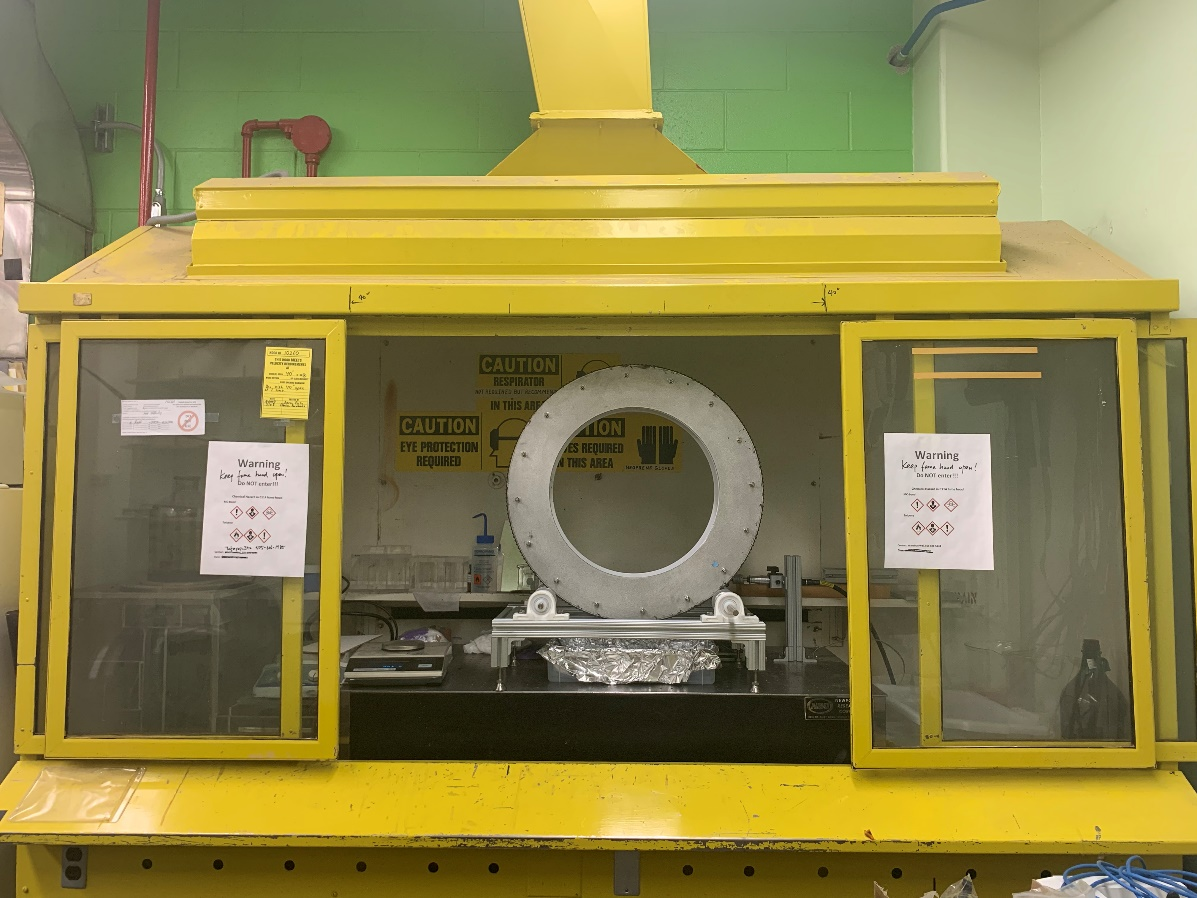
\includegraphics[width=\textwidth]{figures/dPS_jig_and_fume_hood.jpg}
\end{subfigure}%DO NOT REMOVE THIS '%'
\begin{subfigure}{.5\textwidth}
  \centering
  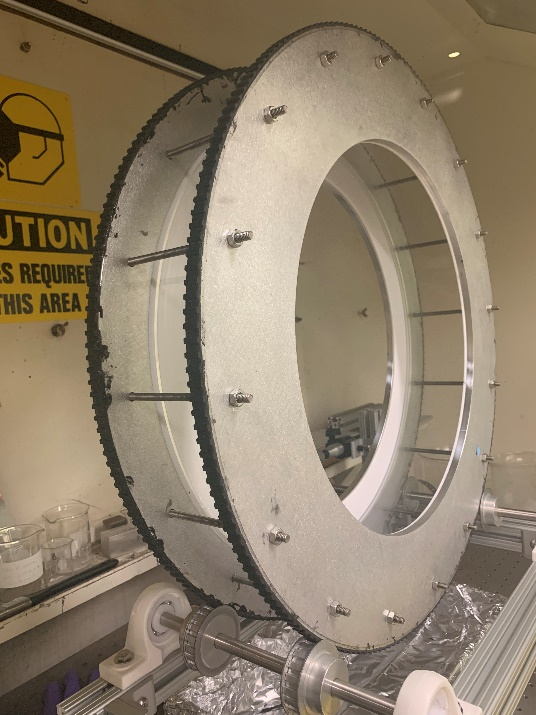
\includegraphics[width=0.57\textwidth]{figures/dPS_jig.jpg}
\end{subfigure}
\caption
{Precession cell wall dPS-coating jig, as described in Sec.~\ref{sec:dPS_coating}}
\label{fig:dPS_coating_jig}
\end{figure}

Two types of dPS-coated PMMA precession cell walls coating methods were used. The first was a manual coating procedure, where the cell wall (oriented such that its central axis was horizontal) was slowly rotated over the course of an hour while a dPS/d-toulene mixture was applied with a brush (that was nonsolvent in toulene). 

The second coating method was the ``rotating lake'' described in Ref.~\cite{bodek_storage_2008}. The cell wall was clamped between two aluminum rings (Fig.~\ref{fig:dPS_coating_jig}), onto which the dPS/d-toulene mixture was poured. This was rotated slowly by a jig at roughly \qty{10}{rpm} for the entirety of the coating and drying process.

For both coating methodologies, \qty{1.5}{\gram} of dPS was dissolved into \qty{0.225}{\liter} d-toulene. The coated cell wall was allowed to dry in a fume hood for \qty{24}{\hour} and then outgassed under vacuum over the course of several days.